%!TEX program = xelatex
\documentclass[12pt,a4paper]{ctexart}

% ------ packages ------
\usepackage{geometry}
\geometry{left=2.5cm, right=2.5cm, top=2.8cm, bottom=2.5cm}
\usepackage{amsmath,amssymb}
\usepackage{graphicx}
\usepackage{booktabs}
\usepackage{multirow}
\usepackage{array}
\usepackage{hyperref}
\usepackage{float}
\usepackage{caption}
\usepackage{enumitem}
\usepackage{fancyhdr}
\usepackage{fontspec}

\hypersetup{
  colorlinks=true,
  linkcolor=blue,
  citecolor=blue,
  urlcolor=blue,
}

\setlength{\parskip}{0.3em plus 0.1em minus 0.1em}
\setlength{\parindent}{2em}
\setlength{\emergencystretch}{2em}

% ------ title ------
\title{{\bfseries 链上数据对加密货币收益率预测的条件有效性研究}}
\author{贺明涵\\{\small 上海第二工业大学\ 计算机与信息工程学院\ 上海\ 201209}\\[2pt]{\small ORCID: 0009-0005-7993-6614}}
\date{}

\begin{document}

\maketitle

% ================================================================
%  中文摘要
% ================================================================
\begin{center}
{\zihao{-4}{\bfseries 摘\ \ 要}}
\end{center}

链上数据被视为加密货币价格预测的重要信息来源，但其在短期收益预测中的有效性缺乏系统检验。本文以比特币4小时级别对数收益率为预测目标，设计六种多源异构特征组合以系统区分短期链上指标（SOPR、CDD）与长期链上指标（交易所余额、活跃地址、净流量）的差异化贡献，在十种覆盖循环、卷积、Transformer、混合架构、线性模型、多尺度混合及树模型的代表性模型上进行公平对比。实验结果表明：（1）短期链上数据不具备独立预测能力——仅与价格特征配合时，所有模型均未取得正测试夏普；但与资金费率和恐慌贪婪指数联合使用后，产生显著的非线性协同增益（$\Delta$Sharpe最高+3.45，跨5种子均值+3.30$\pm$0.69）；长期链上指标（交易所余额、活跃地址、净流量）在4小时频率下未展现预测价值，共同确立了链上数据"条件有效"而非"普遍有效"的核心命题；（2）该协同效应具有显著的架构依赖性——十种模型依其在full集相对price\_funding\_fng集的$\Delta$Sharpe呈现清晰的三组分化：协同利用组（CNN-Transformer、LSTM-Transformer，$\Delta$Sharpe $> +2$）、中性组（Transformer、PatchTST、DLinear、XGBoost，$\Delta$Sharpe $\approx 0$）和负向干扰组（LSTM、TCN、ModernTCN、TimeMixer，$\Delta$Sharpe $< -1.5$），其中TimeMixer作为ICLR 2024 SOTA在fng集上取得全模型最优（Sharpe=4.89）但加入链上后崩溃（$\Delta$ $-$3.11），成为架构依赖性的最强反证；（3）盈亏平衡手续费分析表明混合架构的成本韧性显著优于纯架构（约47 bps vs 27 bps），其行为根源为适中的换手率水平；跨2022--2025年8个市场体制的滑动窗口验证进一步确认了上述分组规律的时间鲁棒性——协同利用组跨窗口夏普均值（3.85）显著优于其他分组，而XGBoost的静态高夏普（4.50）在滑动窗口下完全消失（均值$-0.79$），揭示了单窗口评估可能严重误导模型选择的风险。上述结果表明，链上数据并非普遍具有预测力，其有效性取决于指标类型、配套数据源和模型架构三者的协同匹配。本文的核心贡献在于：揭示了链上数据预测价值的"条件有效性"原理，发现了跨架构的三组分化规律，并建立了一套从预测精度到部署可行性的多维度评估框架。

\vspace{1em}
{\bfseries 关键词：}加密货币；收益预测；链上数据；多源异构数据；深度学习；条件有效性

\vspace{2em}

% ================================================================
%  English Abstract
% ================================================================
\begin{center}
{\zihao{-4}{\bfseries Abstract}}
\end{center}

On-chain data is widely regarded as a valuable information source for cryptocurrency price prediction, yet its effectiveness in short-term return forecasting lacks systematic validation. This paper takes Bitcoin 4-hour log-returns as the prediction target, designs six multi-source heterogeneous feature configurations to systematically isolate the differential contributions of short-term on-chain indicators (SOPR, CDD) versus long-term ones (exchange balance, active addresses, netflow), and conducts a fair comparison across ten models spanning recurrent, convolutional, Transformer, hybrid, linear, multi-scale mixing, and tree-based architectures. Results demonstrate that: (1) short-term on-chain data offers no independent predictive power---when combined only with price features, no model achieves a positive test Sharpe; however, once funding-rate and sentiment features are present, substantial nonlinear synergy emerges ($\Delta$Sharpe up to +3.45, cross-seed mean +3.30$\pm$0.69); long-term on-chain indicators exhibit no predictive power at the 4-hour frequency, establishing the ``conditional effectiveness'' rather than ``universal effectiveness'' of on-chain data; (2) this synergy is strongly architecture-dependent---the ten models separate cleanly into three groups based on their $\Delta$Sharpe from price\_funding\_fng to full: a synergistic-utilization group (CNN-Transformer, LSTM-Transformer; $\Delta$Sharpe $> +2$), a neutral group (Transformer, PatchTST, DLinear, XGBoost; $\Delta$Sharpe $\approx 0$), and a negative-interference group (LSTM, TCN, ModernTCN, TimeMixer; $\Delta$Sharpe $< -1.5$), with TimeMixer (ICLR 2024) achieving the highest Sharpe on price\_funding\_fng (4.89) yet collapsing when on-chain features are added ($\Delta$Sharpe $-$3.11), providing the strongest counterexample to the architecture-dependence thesis; (3) a multi-dimensional evaluation framework combining Diebold--Mariano tests, cost sensitivity analysis, and sliding-window validation across eight market regimes (2022--2025) confirms the temporal robustness of the three-group architecture pattern---the synergistic-utilization group achieves the highest cross-window mean Sharpe (3.85), hybrid architectures exhibit substantially higher cost resilience than pure architectures ($\sim$47 bps vs.\ $\sim$27 bps break-even), and XGBoost's static high Sharpe (4.50) disappears entirely under sliding windows (mean $-0.79$), demonstrating that single-window evaluation can severely mislead model selection. The core contributions are threefold: establishing the ``conditional effectiveness'' principle for on-chain data, discovering the three-group architecture taxonomy for cross-source synergy, and constructing a multi-dimensional evaluation framework spanning prediction accuracy to deployment feasibility. Together, these findings demonstrate that on-chain data's predictive value depends on the three-way alignment of indicator type, companion modalities, and model architecture, carrying implications beyond cryptocurrency forecasting to multi-source heterogeneous data modeling in finance.

\vspace{1em}
{\bfseries Keywords:} cryptocurrency; return prediction; on-chain data; multi-source heterogeneous data; deep learning; conditional effectiveness

\newpage

% ================================================================
%  1. 引言
% ================================================================
\section{引言}

加密货币市场的高波动性和非线性特性使得精准的价格预测极具挑战\cite{urquhart2016,kristoufek2015}。传统时间序列方法如ARIMA和GARCH族模型难以捕捉其复杂动态特征，促使研究者转向深度学习方法。然而，现有研究多聚焦于单一或少数量模型的对比，且对链上数据（on-chain data）这一加密货币市场独有信息源在短期收益预测中的实际有效性缺乏系统检验。已有研究要么将链上数据作为辅助特征直接引入，要么仅在日频或周频层面分析其与价格的长期关系。但一个关键问题仍存在：链上数据的预测价值能否独立存在，还是必须依赖与衍生品信号、市场情绪等其他数据源的协同配合？不同类型链上指标（短期持币者行为指标SOPR/CDD vs 长期供需趋势指标如交易所余额/活跃地址）的差异化价值也未得到区分。

为回答上述问题，本文在比特币4小时K线数据上设计了六种多源异构特征组合，以系统区分链上数据的独立贡献与协同贡献，并在六种架构类别的十种代表性模型上进行公平对比。主要贡献如下：

\begin{enumerate}[label=(\arabic*),leftmargin=2.5em]
    \item 发现条件有效性原理：通过特征消融实验揭示链上数据预测价值的条件性——短期链上指标（SOPR/CDD）在孤立使用时对所有模型均无正向预测能力，但当资金费率和恐慌贪婪指数同时存在时，产生大幅$\Delta$Sharpe增益，在5种子间始终显著（$p<0.05$）；而长期链上指标（交易所余额、活跃地址、净流量）在4小时频率下无预测价值，甚至引入噪声。这一发现确立了链上数据"条件有效"而非"普遍有效"的核心命题。
    \item 发现三组架构分化规律：通过十种模型的交叉对比，发现链上协同效应具有清晰的架构条件依赖性——模型依其对链上数据的利用模式分为三个组别：协同利用组（CNN-Transformer、LSTM-Transformer，$\Delta$Sharpe $>+2$）、中性组（Transformer、PatchTST、DLinear、XGBoost，$\Delta$Sharpe $\approx 0$）和负向干扰组（LSTM、TCN、ModernTCN、TimeMixer，$\Delta$Sharpe $< -1.5$）。TimeMixer（ICLR 2024）在price\_funding\_fng上取得最高Sharpe（4.89），加入链上后反而崩跌（$\Delta$Sharpe $-3.11$），构成架构依赖性的最强反例。DLinear和TimeMixer分别落入中性组和负向干扰组，从架构谱系的极简和最新两端共同确证了该分组的完备性。
    \item 建立多维度评估框架与部署洞察：构建了从预测精度到部署可行性的多维度评估框架（Rank IC、夏普比率、最大回撤、Diebold--Mariano检验、Bootstrap检验、成本敏感性与换手率分析）。发现混合架构的成本韧性约为纯架构的两倍（盈亏平衡约47 bps vs 27 bps）；通过2022--2025年八段滑动窗口验证确认了三类架构分组的时间鲁棒性——协同利用组跨窗口夏普均值3.85；同时发现XGBoost的静态高夏普（4.50）在滑动窗口下完全消失（均值$-0.79$），揭示了单窗口评估可能严重误导模型选择的风险——这对金融预测模型评估具有方法论层面的警示意义。
\end{enumerate}

\section{相关工作}

\subsection{加密货币收益预测}

传统计量经济学方法（如ARIMA、GARCH）在加密货币的高波动场景下表现有限\cite{catania2019,kristoufek2015}。深度学习方法中，LSTM\cite{hochreiter1997}已被广泛用于金融时序预测\cite{mcnally2018}，Transformer的自注意力机制在长距离依赖建模上具有优势\cite{lim2021,wen2023}，其变体PatchTST\cite{nie2023}通过patch分割和通道独立策略在长序列预测上取得领先结果。ModernTCN\cite{luo2024}借鉴现代卷积设计在多个基准上超越Transformer类模型。此外，DLinear\cite{zeng2023}以简单的通道独立线性分解质疑了复杂架构的必要性；TimeMixer\cite{wang2024timemixer}通过多尺度分解混合（PDM+FMM）在ICLR 2024上取得领先结果。本文将这二者纳入，涵盖从"极简线性"到"多尺度混合"的完整架构谱系。

\subsection{多源数据融合与链上数据分析}资金费率反映永续合约多空双方的持仓成本差异\cite{malik2023}，恐慌贪婪指数聚合交易量、波动率、社交媒体情绪等指标量化市场情绪\cite{carosia2024}，两者均与短期价格具有明确的指示逻辑。链上数据则从网络层面揭示供需动态：SOPR（已花费产出利润率）衡量链上移动BTC的加权平均盈亏比，CDD（币天销毁）将交易金额按持币天数加权以识别长期持有者异动。这两类短期链上指标已被用于市场周期转折点识别，但其在4小时级别的短期预测价值尚未被系统检验。长期链上指标（交易所余额、活跃地址、净流量）反映宏观供需趋势，变动周期较长，与4小时频率可能存在粒度不匹配。Alessandretti等人\cite{alessandretti2018}早期验证了区块链衍生特征对加密货币价格预测的潜力，但未系统区分短期与长期链上指标的差异性价值。近期Das等人\cite{das2026}融合Transformer语言模型与图神经网络，结合社交媒体情绪数据预测BTC和ETH价格，验证了情绪信号在多源加密货币预测框架中的价值，但其架构为LSTM-GNN混合体，未涉及链上数据。

已有研究\cite{corbet2019}在链上数据的使用上存在以下不足：（1）未区分短期与长期链上指标在预测粒度上的差异；（2）仅检验独立预测能力，忽略了链上数据可能通过与其他数据源的交互发挥非线性协同效应；（3）未系统研究不同模型架构对链上信号的利用效率差异。Kim等人\cite{kim2022}使用SAM-LSTM（自注意力多分支LSTM）结合链上数据和变点检测预测BTC价格，验证了链上特征的预测潜力，但其未设计特征消融实验来区分链上数据的独立与协同贡献，也未对比不同架构对链上信号的利用差异。

\subsection{现有工作的量化对比与局限}

表\ref{tab:lit_comparison}汇总了近年代表性研究的核心指标，并纳入本文结果进行对比。

\begin{table}[H]
\centering
\caption{近年加密货币收益预测代表性研究的核心指标对比}
\label{tab:lit_comparison}
\small
\begin{tabular}{lcccc}
\toprule
研究 & 模型 & 方向准确率 & 夏普比率 & 其他指标 \\
\midrule
Omole 和 Enke \cite{omole2024} & CNN-LSTM + Boruta & 82.4\% & 6.47 & 年化收益1682\% \\
Kozhevnikov \cite{kozh2025} & XGBoost（全周期） & -- & 1.68 & 最大回撤-17.3\% \\
Kozhevnikov \cite{kozh2025} & LSTM & 52.4\% & -- & -- \\
Kim et al.\ \cite{kim2022} & SAM-LSTM & -- & -- & 链上数据+CPD \\
高维指标融合 \cite{findev2025} & XGBoost（BTC） & 55.9\% & 1.78 & 累积收益141.4\% \\
Pambudi et al.\ \cite{pambudi2025} & Transformer & -- & -- & MAPE 0.20\% \\
\textbf{本文} & \textbf{CNN-Transformer} & \textbf{54.7\%} & \textbf{5.19} & \textbf{IC=0.150} \\
\bottomrule
\multicolumn{5}{l}{\small 注：（1）各研究的数据周期、频率、交易成本设定不同，以上数字不可直接等价比较；} \\
\multicolumn{5}{l}{\small （2）Omole和Enke使用2012--2023日频数据，涵盖完整牛熊周期；本文使用4小时频率；} \\
\multicolumn{5}{l}{\small （3）IC（信息系数）在加密货币文献中鲜有报告，本文引入该指标作为补充。}
\end{tabular}
\end{table}

从表\ref{tab:lit_comparison}可以看出，本文CNN-Transformer的方向准确率（54.7\%）较文献LSTM典型值（52.4\%）有小幅提升。但各研究的数据周期、频率和成本设定不同，且不同频率下的夏普比率不可直接比较——高频策略的年化夏普因样本量较大而天然偏高，以上数字不可等价对比。综合现有工作，仍缺乏在统一框架下对混合与纯架构的公平对比，链上数据的特征消融多以"叠加"方式验证、未区分协同效应与架构依赖性，且评估多停留在MSE层面、IC指标几乎未被使用。

\section{数据与特征工程}

\subsection{数据来源与预处理}

本文使用的原始数据包含以下来源：

\begin{itemize}[leftmargin=2.5em]
    \item 价格与交易量数据：来自币安交易所的BTC/USDT永续合约1小时K线数据（经4小时重采样），包含开盘价、最高价、最低价、收盘价和交易量。
    \item 资金费率：对应时间窗口的永续合约资金费率数据。
    \item 恐慌贪婪指数：来自Alternative.me，反映市场情绪的每日数据，按4小时频率前向填充。
    \item 链上指标：来自Dune Analytics和OKLink，包括SOPR（已花费产出利润率）、CDD（币天销毁）、交易所BTC余额、活跃地址数和BTC净流量。
\end{itemize}

所有数据按时间对齐并合并为4小时频率的统一数据集，缺失值采用前向填充处理。最终数据集覆盖2020年1月1日至2026年5月7日（4小时频率，共13,909条原始记录）。按时间顺序划分为训练集（2020年1月--2024年6月，9,736条，70\%）、验证集（2024年6月--2025年6月，2,086条，15\%）与测试集（2025年6月--2026年5月，2,087条，15\%）。经$L=48$回溯窗口构建序列后，实际样本数为训练集9,702条、验证集2,079条、测试集2,080条。

\subsection{特征构建}

\subsubsection{价格形态特征}

对每个滞后步长$l \in \{1,2,3,4,6,8,12\}$计算对数收益率：
\begin{equation}
\text{ret}_l = \ln \frac{\text{close}_t}{\text{close}_{t-l}}
\end{equation}

还包括收益加速度（两个不同滞后期收益的差）、对数成交量及其变动率，以及基于最高价和最低价计算的价格位置指标（HH、LL和价格位置比）。

\subsubsection{多尺度统计特征}

对每个连续型因子，在窗口$w \in \{4,8,12,24\}$上计算：
\begin{equation}
z_w = \frac{x_t - \mu_w}{\sigma_w + \epsilon}
\end{equation}
\begin{equation}
\text{mom}_w = \frac{x_t}{x_{t-w}} - 1
\end{equation}
分别代表标准化偏离和窗口期动量。

\subsubsection{链上特征构建与选取逻辑}

SOPR和CDD作为短期链上代表，各构建11维特征（原始值/对数变换、一阶及二阶差分、4窗口z-score和动量，共22维）。交易所BTC余额、活跃地址数和净流量作为长期链上代表，变动周期以日或周为单位，纳入price\_long\_onchain特征集以检验其短期预测价值，并在full特征集中予以排除（经预实验验证未带来增益）。

\subsubsection{跨源交互特征}

本文构建了四类乘积交互项以捕捉数据源间的非线性耦合：情绪--盈亏比（fng\_sopr\_int）、大户异动--成交量（cdd\_vol\_int）、资金费率--波动率（fr\_vol\_int）和极端情绪--动量（fng\_mom\_int）。其中前两者依赖SOPR/CDD数据，仅存在于full集。因此full集相较price\_funding\_fng的24维增量中，22维为原始链上特征，2维为新增链上依赖型交互项。原始链上特征赋予模型比固定乘积更灵活的跨源组合自由度（详见第6.2节）。

\subsection{特征组合设计（消融实验）}

为系统评估不同来源信息对预测的贡献——特别是链上数据的独立价值与协同价值——本文设计了六种特征组合，如表\ref{tab:feature_sets}所示。这六种组合的逻辑并非简单的逐层叠加，而是服务于三个递进的分析目标：（1）通过price\_only建立纯价格基线；（2）通过price\_onchain和price\_long\_onchain检验链上数据在"仅配合价格"时的独立预测能力；（3）通过price\_funding\_fng与full的对比，检验链上数据在"已有衍生品和情绪数据"基础上的增量协同效应。若full显著优于price\_funding\_fng，且price\_onchain表现不佳，则说明链上数据的价值不是独立的，而是条件性的——依赖于与其他数据源的交互。

\begin{table}[H]
\centering
\caption{六种特征组合及其包含的数据源}
\label{tab:feature_sets}
\begin{tabular}{lcccc}
\toprule
\multirow{2}{*}{特征组合} & \multicolumn{4}{c}{数据源} \\
\cmidrule(lr){2-5}
& 价格 & 资金费率 & 恐慌贪婪 & 链上 \\
\midrule
price\_only        & \checkmark & & & \\
price\_funding     & \checkmark & \checkmark & & \\
price\_funding\_fng & \checkmark & \checkmark & \checkmark & \\
price\_onchain     & \checkmark & & & \checkmark \\
price\_long\_onchain & \checkmark & & & \checkmark* \\
full               & \checkmark & \checkmark & \checkmark & \checkmark \\
\bottomrule
\multicolumn{5}{l}{\small *仅price\_long\_onchain包含长期链上指标（交易所余额、活跃地址、净流量）；} \\
\multicolumn{5}{l}{\small full中的链上特征为SOPR和CDD，长期链上指标经测试因表现不佳未纳入} \\
\end{tabular}
\end{table}

序列构建采用滑动窗口方式，回溯窗口$L=48$（即过去48个4小时K线，约8天），预测窗口$H=1$（下个4小时的对数收益率）。各特征组合维度分别为：price\_only 18维、price\_funding 28维、price\_funding\_fng 40维、price\_onchain 40维、price\_long\_onchain 48维、full 64维。

数据集按时间顺序划分为训练集（前70\%）、验证集（中间15\%）和测试集（后15\%）。特征标准化采用鲁棒标准化（RobustScaler，5\%--95\%分位数），以减轻极端值对深度学习训练的影响。标准化器仅在训练集上拟合（fit\_transform），验证集和测试集仅应用变换（transform），以避免未来信息泄露。

\subsection{时序完整性验证}

金融时序预测中，训练集与测试集之间的前瞻偏差（look-ahead bias）是导致回测结果虚高的首要原因。本文从三个层面确保时序完整性，杜绝未来信息泄露。

\textbf{（1）时序切分与标准化。}数据集严格按时间顺序划分为训练集、验证集和测试集，未进行随机打乱。RobustScaler仅在训练集上拟合，验证集和测试集仅应用变换，杜绝标准化环节的信息跨集流动。

\textbf{（2）特征构造的因果约束。}所有特征均仅依赖当前及历史信息：滚动统计量（z-score、动量）使用pandas默认的后视窗口（\texttt{rolling}），差分与滞后项使用\texttt{diff()}和\texttt{shift(lag)}（均为后视操作），缺失值采用前向填充（\texttt{ffill}，仅使用过去值）。预测目标$\text{ret}_{t+1} = \ln(\text{close}_{t+1} / \text{close}_t)$作为独立标签列存储，未参与任何特征构造。

\textbf{（3）序列构建的索引边界。}滑动窗口序列构建时，对每个时间索引$i$，特征窗口严格取$[i-L, i-1]$区间，标签取第$i$步的目标值。训练/验证/测试集的序列划分在索引维度上连续且无重叠。

以上设计确保了本文所有实验结果均不包含前瞻偏差。完整的数据处理与训练代码已随论文公开，供复现验证。

\section{模型方法}

\subsection{模型总览}

本文对比了以下十种模型，涵盖六大类别，详细超参数见表\ref{tab:model_config}：

\begin{itemize}[leftmargin=2.5em]
    \item 循环神经网络：双层单向LSTM\cite{hochreiter1997}（隐层192维），作为RNN类基准。
    \item Transformer：标准Transformer编码器\cite{vaswani2017}（d\_model=192，4头，2层）及PatchTST\cite{nie2023}（patch\_len=8，stride=2，通道联合嵌入）。
    \item 卷积网络：TCN\cite{bai2018}（2层残差因果卷积，kernel=3，隐层96维）及ModernTCN\cite{luo2024}（3层，kernel=31，BatchNorm+GELU）。
    \item 混合架构：CNN-Transformer（3层因果卷积→Transformer编码器，12头注意力）及LSTM-Transformer（双层LSTM→Transformer编码器），均为d\_model=192。
    \item 线性模型：DLinear\cite{zeng2023}（移动平均核=13，通道独立），作为"简单即有效"范式的代表——若线性模型在复杂特征空间中仍能取得竞争力表现，则对深层架构的必要性提出质疑。
    \item 多尺度混合：TimeMixer\cite{wang2024timemixer}（d\_model=128，4尺度分解，2个PDM块，FMM集成），作为ICLR 2024最新多尺度时序混合架构的代表。
    \item 树模型：XGBoost\cite{chen2016}（学习率0.05，最大深度5，2000棵树），作为传统机器学习基准。
\end{itemize}

\begin{table}[H]
\centering
\footnotesize
\setlength{\tabcolsep}{1.8pt}
\caption{各模型核心超参数配置}
\label{tab:model_config}
\begin{tabular}{lcccccc}
\toprule
模型 & 隐层维度 & 层数 & 头数/核大小 & Dropout & 学习率 & 参数量 \\
\midrule
LSTM & 192 & 2 & -- & 0.13 & 1e-4 & 0.49M \\
Transformer & 192 & 2 & 4 & 0.13 & 1e-4 & 0.46M \\
TCN & 96 & 2 & 3 & 0.13 & 1e-4 & 0.11M \\
CNN-Transformer & 192 & 2+3 & 12 / 5 & 0.13 & 1e-4 & 1.75M \\
LSTM-Transformer & 192 & 2+2 & 4 & 0.13 & 1e-4 & 1.21M \\
PatchTST & 192 & 2 & 8 & 0.13 & 1e-4 & 0.71M \\
ModernTCN & 96 & 3 & 31 & 0.13 & 1e-4 & 0.22M \\
DLinear & -- & -- & 13 (MA核) & -- & 1e-4 & 0.006M \\
TimeMixer & 128 & 2$\times$PDM & 4 (尺度数) & 0.13 & 1e-4 & 2.28M \\
XGBoost & -- & -- & -- & -- & 0.05 & 2000棵树 \\
\bottomrule
\multicolumn{7}{p{\textwidth}}{\footnotesize CNN-Transformer的"2+3"表示2层Transformer + 3层卷积；DLinear的参数量以full特征集（64维）计；TimeMixer的"2$\times$PDM"表示2个Past-Decomposable-Mixing块。}
\end{tabular}
\end{table}

CNN-Transformer的详细架构如图\ref{fig:cnn_transformer_arch}所示。

\begin{figure}[H]
\centering
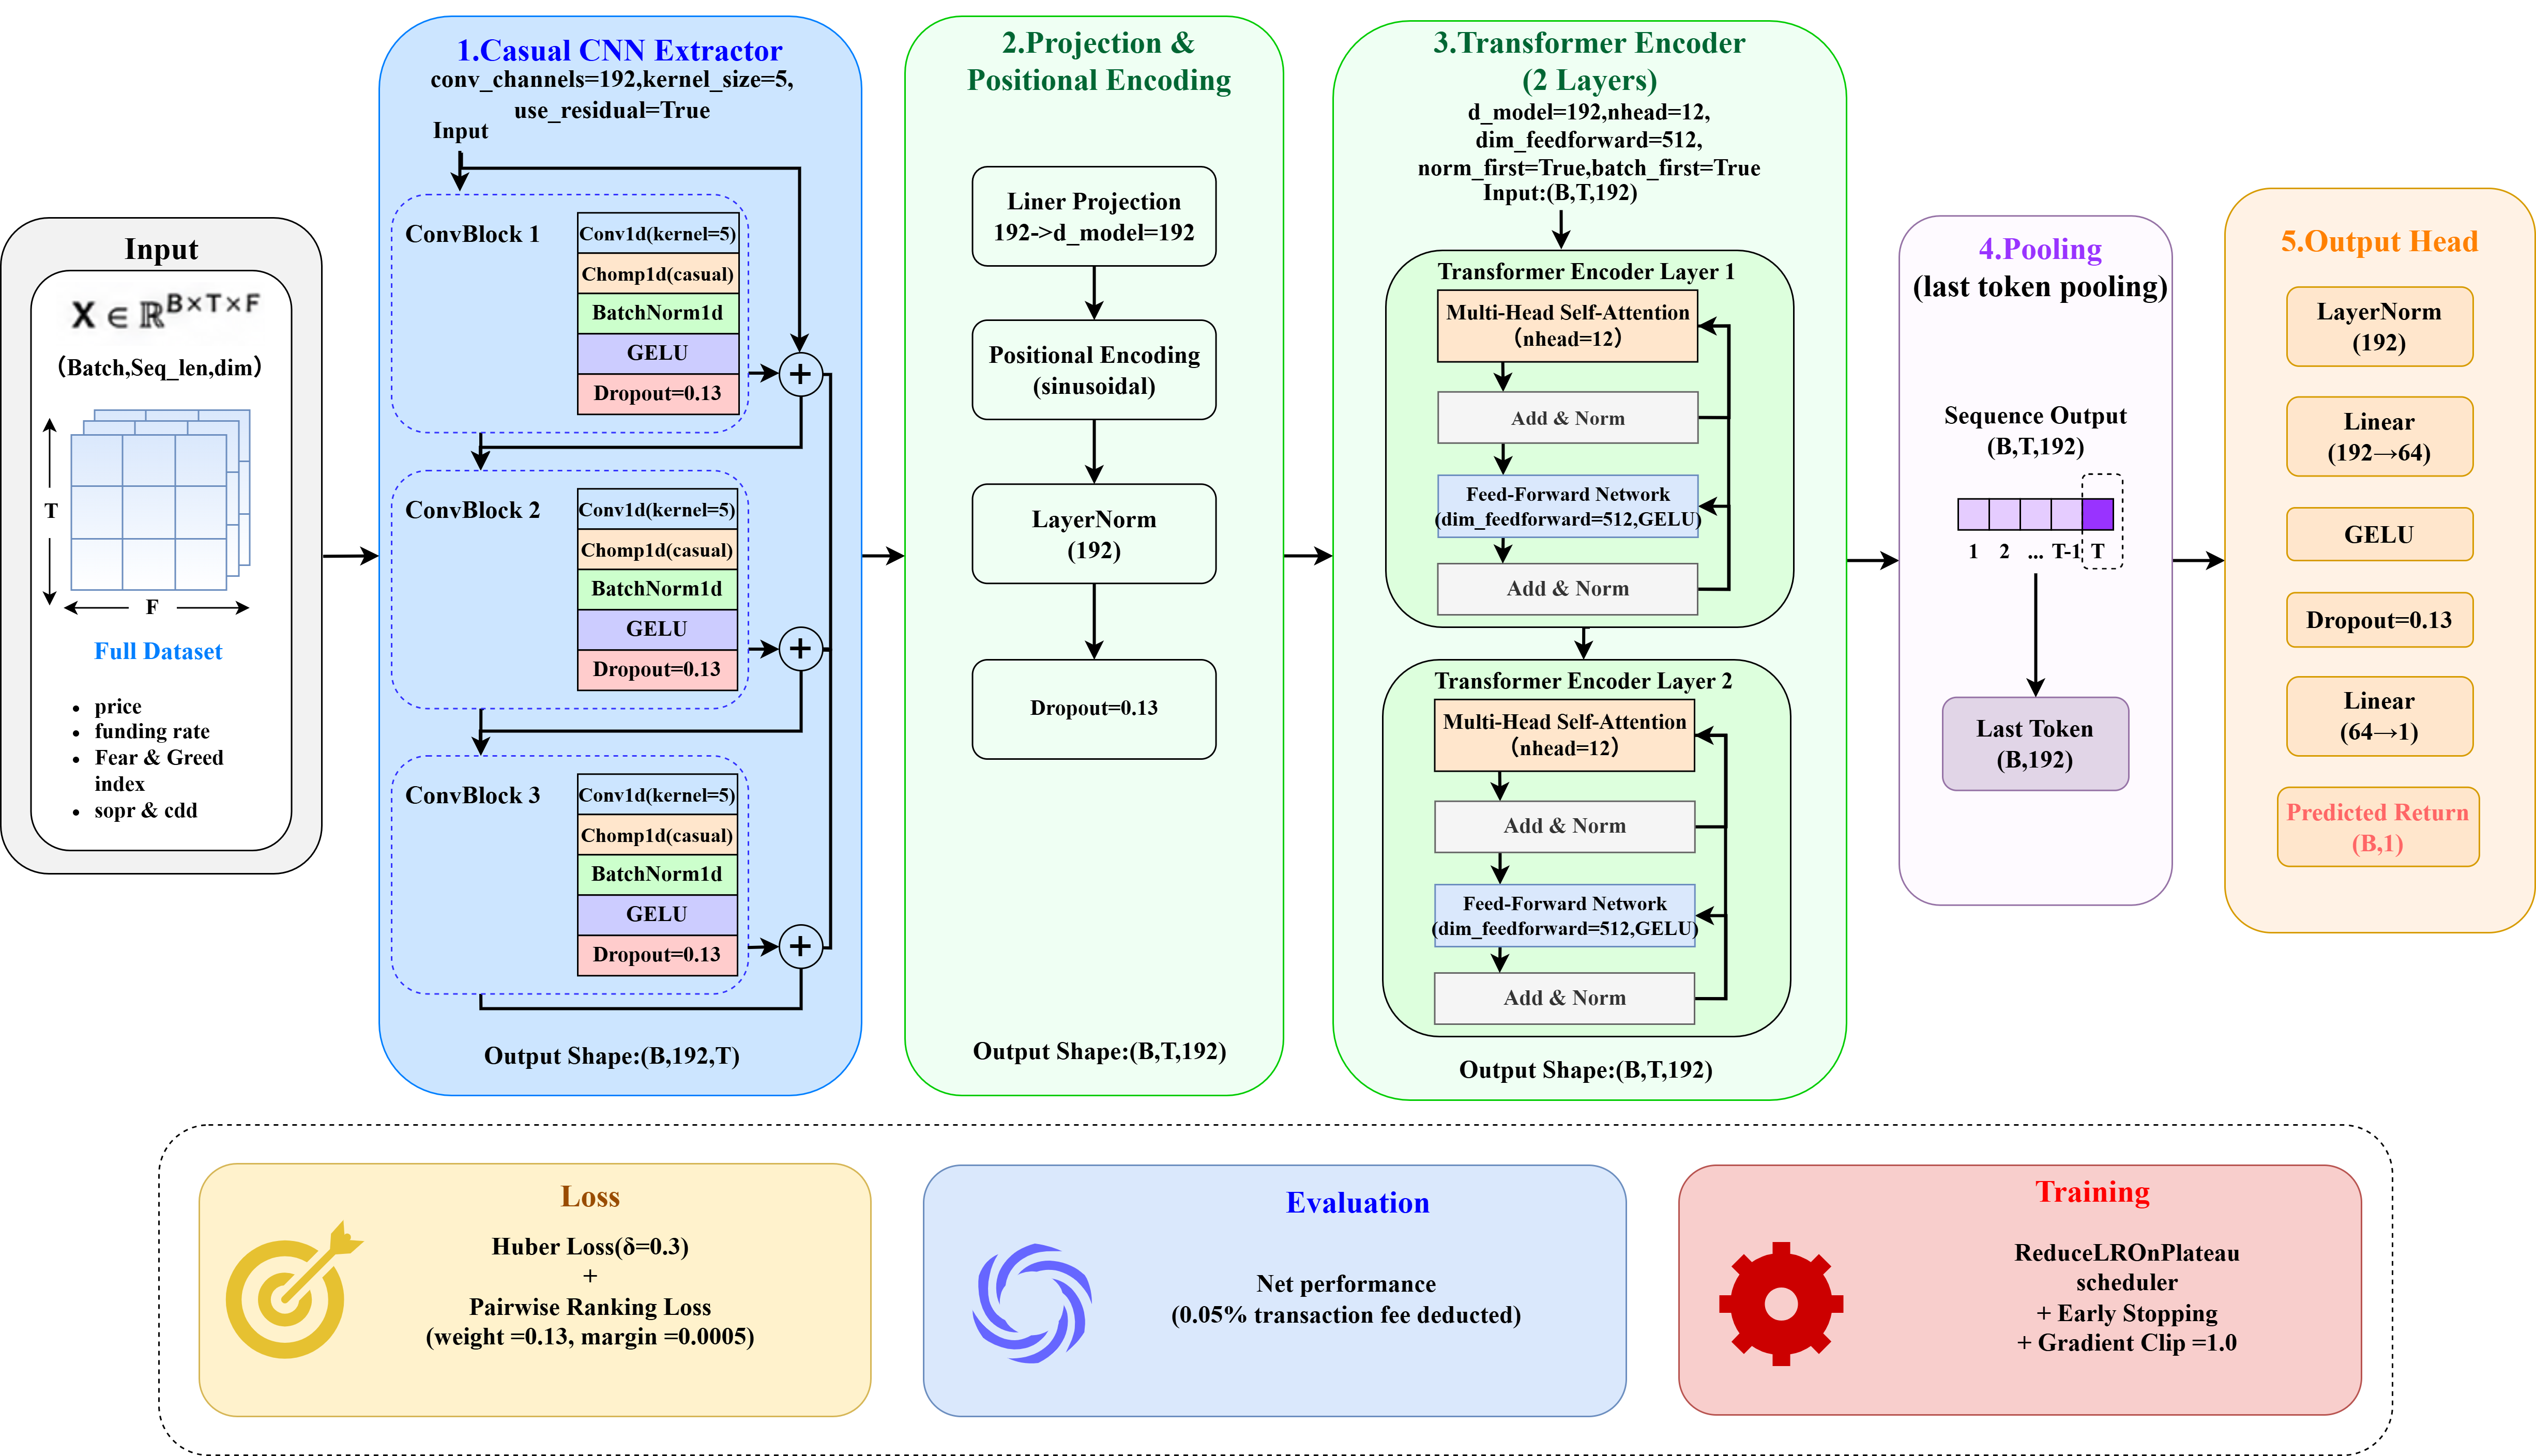
\includegraphics[width=0.78\textwidth]{../charts/CNN-Transformer.png}
\caption{CNN-Transformer模型架构：输入序列经三层因果卷积（ConvBlock）提取局部模式，再由Transformer编码器捕捉长距离依赖，最后通过池化层输出对数收益率预测}
\label{fig:cnn_transformer_arch}
\end{figure}

\subsection{损失函数设计}

借鉴量化金融中的排序学习（learning-to-rank）理念，本文设计了一种组合损失函数，兼顾预测值的绝对精度和样本间的相对排序。总损失函数如下：

\begin{equation}
\mathcal{L} = (1 - \lambda_{\text{rank}}) \cdot \mathcal{L}_{\text{Huber}} + \lambda_{\text{rank}} \cdot \mathcal{L}_{\text{Ranking}}
\end{equation}

其中$\mathcal{L}_{\text{Huber}}$为Huber损失（$\delta=0.3$），对极端离群值具有鲁棒性；$\mathcal{L}_{\text{Ranking}}$为Margin Ranking Loss：

\begin{equation}
\mathcal{L}_{\text{Ranking}} = \frac{1}{N}\sum_{(i,j)} \max\left(0, -\text{sign}(y_i - y_j) \cdot (\hat{y}_i - \hat{y}_j) + m\right)
\end{equation}

该损失惩罚预测排序与真实排序不一致的样本对，$m=0.0005$为排序间隔。在量化交易中，准确的相对排序往往比精确的绝对值更为重要，只要预测方向正确，交易策略即可获利。排序损失权重$\lambda_{\text{rank}}=0.13$。上述三个超参数（$\delta$、$\lambda_{\text{rank}}$、$m$）均通过验证集网格搜索确定，选最终验证损失最低的组合。

\subsection{训练设置}

所有深度学习模型统一采用以下训练配置：批量大小64，AdamW优化器，权重衰减1e-4，最大训练轮次200，早停耐心值20轮，学习率调度器采用ReduceLROnPlateau（mode='min', factor=0.5, patience=10），梯度裁剪阈值1.0。预测值在评估时裁剪至$[-0.005, 0.005]$区间，以剔除极端预测值对策略指标的干扰。

\section{实验设计}

\subsection{评估指标}

本文从预测能力和策略表现两个维度建立评估体系。预测能力维度包含：

\begin{itemize}[leftmargin=2.5em]
    \item Rank IC（IC）：预测值与真实值之间的Spearman等级相关系数，衡量预测的排序准确性。
    \item Pearson IC（PIC）：预测值与真实值之间的Pearson线性相关系数。
    \item 方向准确率（DA）：预测方向（正/负）与真实方向一致的样本比例。
    \item 均方误差（MSE）：预测值与真实值之间的均方误差。
\end{itemize}

策略表现维度基于一个模拟交易策略计算：当预测值为正时做多，为负时做空，持仓规模为$\text{sign}(\hat{y})$，并考虑0.05\%（5 bps）的双边交易成本。在此基础上计算：

\begin{itemize}[leftmargin=2.5em]
    \item 夏普比率（Sharpe）：年化夏普比率，时间频率换算系数为2190（年化4小时周期数）。
    \item 信息比率（IR）：基于48期滚动Rank IC的均值与标准差之比，衡量信号一致性\cite{grinold2000}。
    \item 最大回撤（MaxDD）：模拟权益曲线的最大回撤幅度。
    \item 年化收益（Annual Return）：年化后的策略平均收益。
\end{itemize}

\subsection{实验设置}

本文设计了以下四组实验：

\begin{enumerate}[label={实验\arabic*：},leftmargin=2.5em]
    \item 全特征集模型对比：在full特征集上对比全部10个模型的测试集表现，检验不同架构的预测能力。
    \item 特征消融实验：在6种特征组合上分别训练10个模型，分析不同来源特征对预测的边际贡献。
    \item 多种子稳定性分析：使用5个不同随机种子（0, 1, 2, 42, 123）重复实验，检验结论的统计可靠性。
    \item 滑动窗口验证实验：采用固定大小滑动窗口（训练2年/测试6个月/步长6个月，共8个窗口，seed=1）在full特征集上训练全部10个模型，检验不同市场趋势下的模型鲁棒性。
\end{enumerate}

\section{实验结果与分析}

\subsection{全特征集模型对比}

表\ref{tab:full_results}展示了全部10个模型在full特征集上（seed=1）的测试集完整评估结果。

\begin{table}[H]
\centering
\footnotesize
\setlength{\tabcolsep}{2pt}
\caption{全特征集（full）各模型测试集表现对比（seed=1）}
\label{tab:full_results}
\begin{tabular}{lcccccccc}
\toprule
模型 & IC & PIC & DA & MSE & Sharpe & IR & MaxDD & AnnRet \\
\midrule
CNN-Transformer & \bfseries0.149 & \bfseries0.163 & \bfseries0.549 & 0.0001 & \bfseries5.652 & \bfseries1.125 & 0.186 & \bfseries2.306 \\
LSTM-Transformer & 0.108 & 0.131 & 0.530 & 0.0001 & 3.259 & 0.865 & 0.255 & 1.334 \\
Transformer & 0.135 & 0.151 & 0.545 & 0.0001 & 4.333 & 0.989 & 0.207 & 1.773 \\
LSTM & 0.119 & 0.120 & 0.519 & 0.0001 & 2.257 & 0.992 & 0.291 & 0.925 \\
TCN & 0.062 & 0.085 & 0.512 & 0.0001 & 0.050 & 0.494 & 0.366 & 0.021 \\
ModernTCN & 0.063 & 0.083 & 0.513 & 0.0001 & 0.168 & 0.455 & 0.415 & 0.069 \\
PatchTST & 0.128 & 0.145 & 0.532 & 0.0001 & 3.981 & 0.867 & 0.261 & 1.630 \\
DLinear & 0.051 & 0.063 & 0.520 & 0.0001 & $-$0.464 & 0.331 & 0.490 & $-$0.191 \\
TimeMixer & 0.115 & 0.147 & 0.524 & 0.0001 & 1.781 & 0.790 & 0.321 & 0.730 \\
XGBoost & 0.128 & 0.144 & 0.542 & 0.0001 & 4.496 & 0.885 & 0.183 & 1.838 \\
\midrule
买入持有 & -- & -- & -- & -- & -0.710 & -- & 0.518 & -0.292 \\
简单动量 & -- & -- & 0.481 & -- & 0.290 & -- & -- & 0.119 \\
\bottomrule
\end{tabular}
\end{table}

从表\ref{tab:full_results}可以观察到以下核心发现：

全部10个模型均显著优于朴素基准：买入持有夏普-0.71（BTC在测试期高位震荡回调），排除了模型正收益来自市场Beta暴露的可能。

（1）CNN-Transformer在数值上表现最优，Transformer和XGBoost紧随其后。CNN-Transformer在多数指标上取得最佳结果（Sharpe=5.65, IC=0.149）。Transformer（4.33）、XGBoost（4.50）和PatchTST（3.98）也取得较强结果。需注意XGBoost的静态高夏普在滑动窗口下不可复现（见第6.6节）。DLinear作为线性基线，在full集上测试夏普为负（$-$0.46），表明简单线性分解无法在此多源异构、低信噪比场景下提取有效信号——深层架构是必要的。TimeMixer（ICLR 2024）在full集上测试夏普1.78，显著弱于其price\_funding\_fng集上的表现（4.89），该剧烈衰减（$\Delta$Sharpe $-$3.11）揭示了一个关键现象：即使是最新的多尺度混合架构，若缺乏层级化特征提取（CNN局部→Transformer全局），也无法有效利用链上数据。ModernTCN和TCN表现出严重的训练-测试性能鸿沟——以ModernTCN为例，seed=1训练集夏普高达19.30，测试集仅0.17，提示纯卷积架构在此低信噪比场景下存在结构性不足（跨种子及训练集详细统计见第6.3节）。

（2）IC的微小提升可非线性放大为夏普比率的可观改善。CNN-Transformer与Transformer的IC差异（0.149 vs 0.135）相对温和，但Sharpe数值差距（5.65 vs 4.33）在量化交易实践中具有经济意义——小幅排序精度的改善可能转化为显著的策略收益差异。

\begin{figure}[H]
\centering
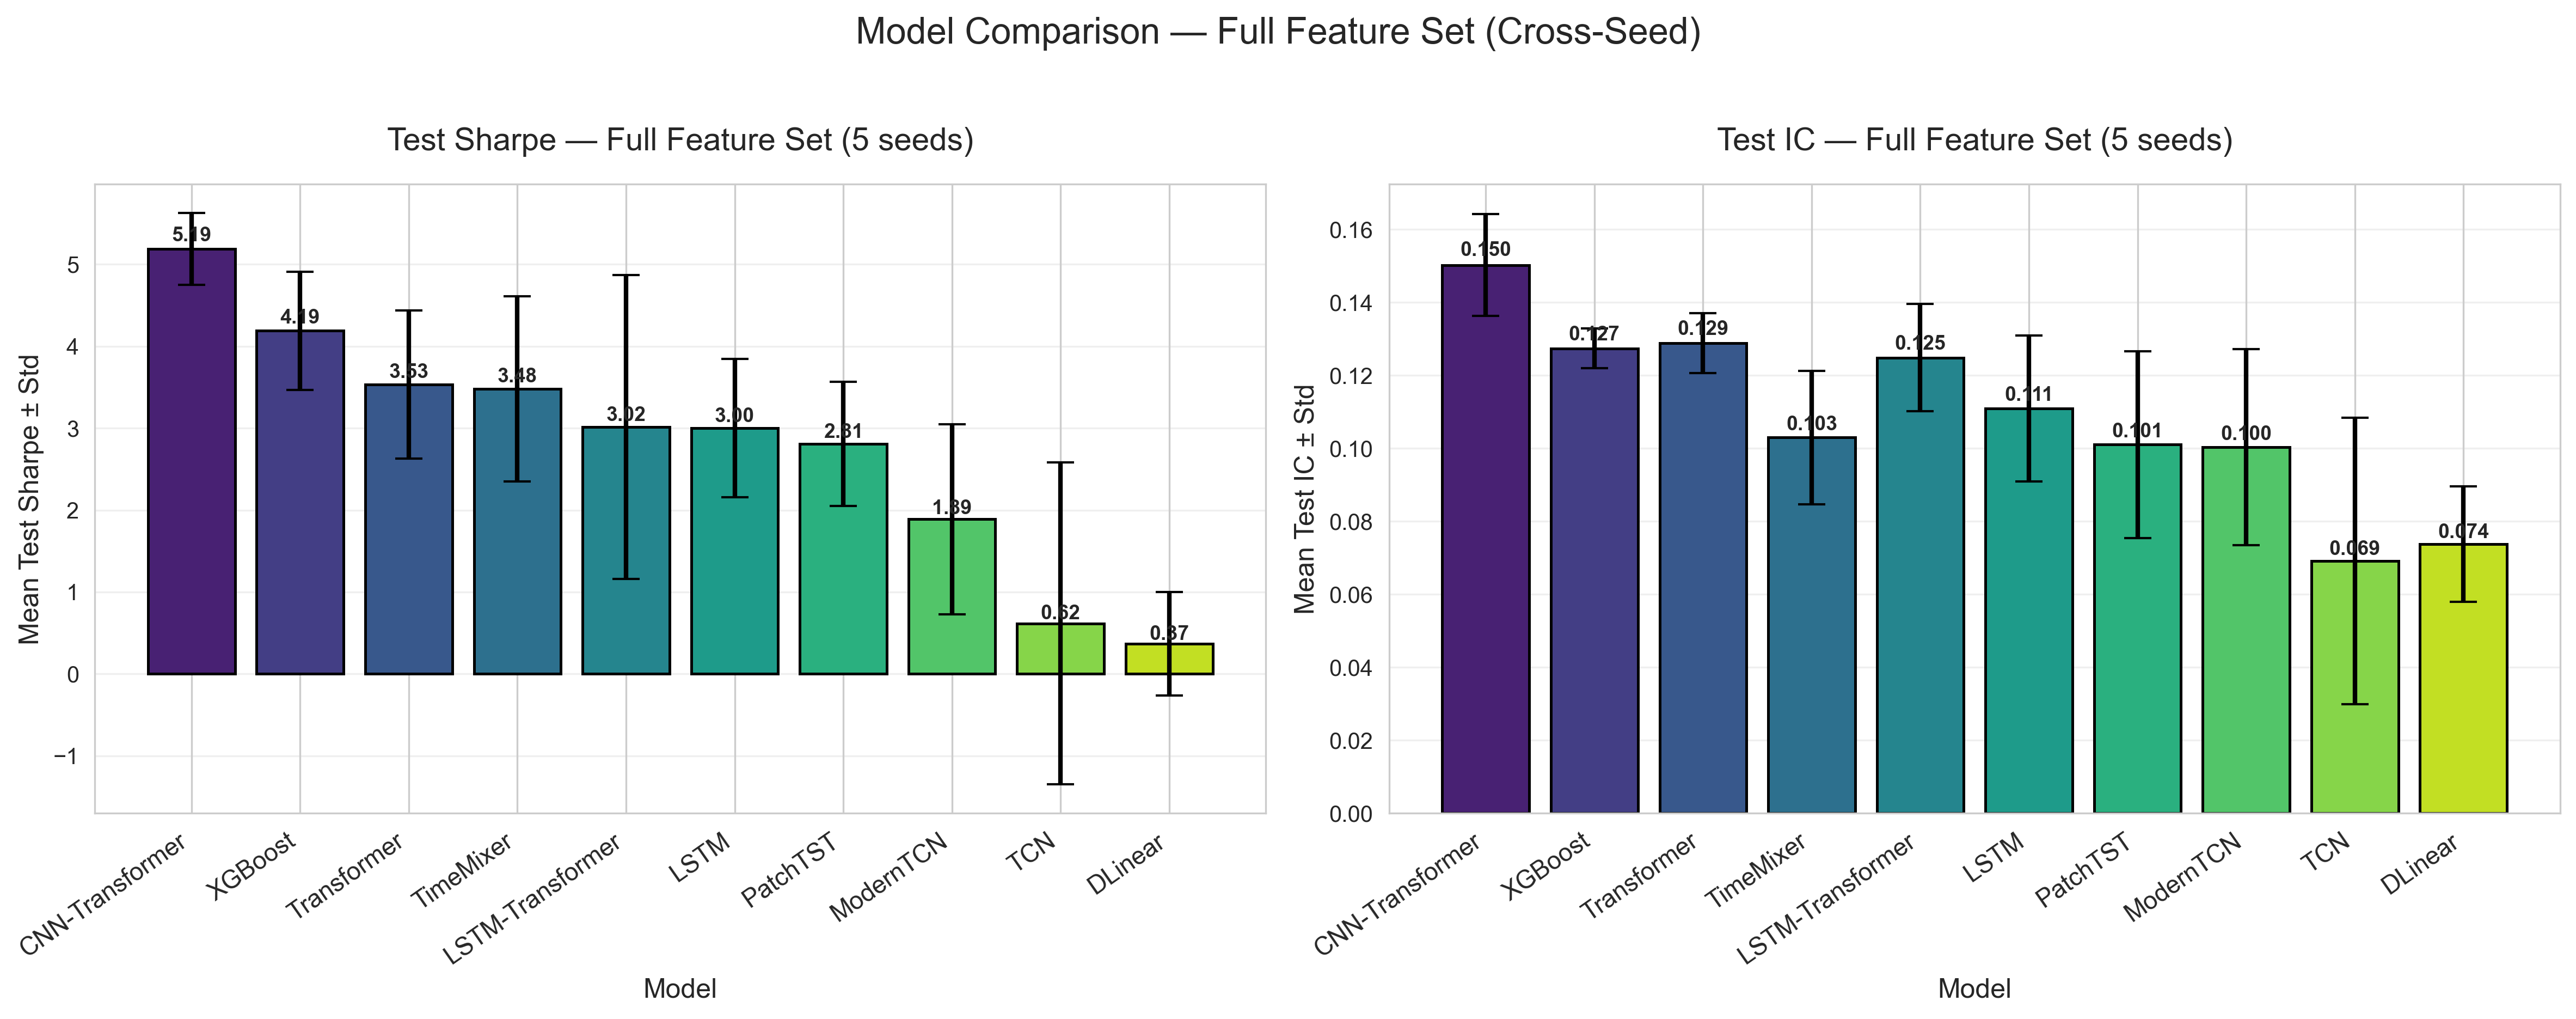
\includegraphics[width=0.80\textwidth]{../charts/model_comparison_full.png}
\caption{全特征集下各模型跨5种子的测试集夏普比率与IC对比（均值$\pm$标准差）}
\label{fig:model_comparison}
\end{figure}

\subsection{特征消融实验}

表\ref{tab:feature_ablation}展示了6种特征组合下各模型测试集的夏普比率，以及同模型跨特征集的排名情况。

\begin{table}[H]
\centering
\footnotesize
\setlength{\tabcolsep}{1.5pt}
\caption{各模型在六种特征组合下的测试集夏普比率对比（seed=1）}
\label{tab:feature_ablation}
\begin{tabular}{lcccccccc}
\toprule
\multirow{2}{*}{模型} & \multicolumn{6}{c}{特征组合} & \multirow{2}{*}{均值} & \multirow{2}{*}{标准差} \\
\cmidrule(lr){2-7}
& only & fund & fng & onch & lon & full \\
\midrule
CNN-Transformer & -2.27 & -2.52 & 2.20 & -0.85 & -2.90 & \bfseries5.65 & -0.11 & 3.26 \\
Transformer & -1.94 & -2.00 & 4.37 & -1.42 & -2.70 & \bfseries4.33 & 0.11 & 3.14 \\
LSTM & -1.10 & -0.19 & 4.28 & -2.01 & -1.87 & \bfseries2.26 & 0.23 & 2.60 \\
LSTM-Transformer & -0.07 & -0.81 & 0.46 & -0.94 & -1.94 & \bfseries3.26 & -0.01 & 1.81 \\
TCN & -2.79 & -3.31 & 1.75 & -3.11 & -2.76 & \bfseries0.05 & -1.70 & 2.36 \\
ModernTCN & -2.35 & -1.20 & 2.39 & -3.69 & -0.61 & \bfseries0.17 & -0.88 & 2.10 \\
PatchTST & -1.44 & -3.29 & 3.52 & -0.73 & -2.68 & \bfseries3.98 & -0.11 & 3.12 \\
DLinear & -2.72 & -2.66 & 0.82 & -2.68 & -2.83 & \bfseries$-$0.46 & -1.75 & 1.52 \\
TimeMixer & -1.46 & -0.44 & \bfseries4.89 & -0.71 & -1.63 & \bfseries1.78 & 0.41 & 2.72 \\
XGBoost & -- & -- & 4.50 & -- & -- & \bfseries4.50 & -- & -- \\
\bottomrule
\multicolumn{9}{p{\textwidth}}{\footnotesize 注：only=price\_only; fund=price\_funding; fng=price\_funding\_fng; onch=price\_onchain; lon=price\_long\_onchain; full=全特征。XGBoost在其余特征集上收敛失败（IC=0），以``--''表示。DLinear在price\_funding\_fng上可取得正Sharpe（0.82），但显著弱于深度模型；TimeMixer在price\_funding\_fng上取得全模型最高Sharpe（4.89），但加入链上数据后大幅衰减至1.78（$\Delta$ $-$3.11），详见第6.2节分析。}
\end{tabular}
\end{table}

从表\ref{tab:feature_ablation}可以观察到一个反直觉的现象：链上数据在孤立使用时对大多数模型没有帮助，但在正确的组合中却产生巨大增益。

当链上指标仅与价格特征配合时，所有模型均未取得正测试夏普。price\_onchain和price\_long\_onchain在所有10个模型上均未产生正收益。以CNN-Transformer为例，加入链上数据后Sharpe从-2.27升至-0.85（有所改善但仍为负值）；而LSTM、TCN和ModernTCN在加入链上数据后反而恶化（如TCN从-2.79降至-3.11）。DLinear在所有特征组合上均表现羸弱（最优仅price\_funding\_fng上Sharpe=0.82），其通道独立线性分解无法捕获跨源非线性交互。原因有三：链上指标的变动逻辑倾向于日频以上，与4小时粒度不匹配；链上交易的随机性掩盖了系统性信号；短期价格主要由衍生品市场博弈而非链上供需驱动。

然而，一旦衍生品和情绪特征同时存在，情况便截然不同。TimeMixer在此三源组合下取得全模型最高夏普（4.89），超越了所有深度模型，表明其多尺度分解混合机制在价格+衍生品+情绪的特征空间中具有出色预测力。表\ref{tab:onchain_synergy}以price\_funding\_fng为基准，对比了各模型在full上的夏普变化。

\begin{table}[H]
\centering
\caption{链上数据协同效应：从price\_funding\_fng到full的夏普比率变化（seed=1）}
\label{tab:onchain_synergy}
\small
\begin{tabular}{lcccc}
\toprule
模型 & Sharpe$_{\text{fng}}$ & Sharpe$_{\text{full}}$ & $\Delta$Sharpe & 协同类型 \\
\midrule
CNN-Transformer & 2.20 & 5.65 & +3.45 & 强正向协同 \\
LSTM-Transformer & 0.46 & 3.26 & +2.80 & 强正向协同 \\
PatchTST & 3.52 & 3.98 & +0.46 & 弱正向协同 \\
Transformer & 4.37 & 4.33 & $-$0.04 & 中性 \\
XGBoost & 4.50 & 4.50 & 0.00 & 完全无视 \\
DLinear & 0.82 & $-$0.46 & $-$1.28 & 弱负向/近中性 \\
TCN & 1.75 & 0.05 & $-$1.70 & 负向干扰 \\
LSTM & 4.28 & 2.26 & $-$2.02 & 负向干扰 \\
ModernTCN & 2.39 & 0.17 & $-$2.22 & 负向干扰 \\
TimeMixer & \bfseries4.89 & 1.78 & \bfseries$-$3.11 & 强负向干扰 \\
\bottomrule
\end{tabular}
\end{table}

CNN-Transformer的测试夏普增加了3.45个点（2.20$\to$5.65），LSTM-Transformer增加了2.80（0.46$\to$3.26）。然而同样的链上特征却损害了LSTM、TCN和ModernTCN，对Transformer和PatchTST几乎无影响，而XGBoost则完全不予利用（$\Delta$Sharpe=0）。最引人注目的是TimeMixer的崩溃：在price\_funding\_fng上以全模型最高夏普4.89领先，但加入链上数据后暴跌至1.78（$\Delta$ $-$3.11），原因是其跨尺度混合发生在时间维度而非特征维度，缺乏对跨源关系的显式建模。

这些结果清晰地映射到架构族，10个模型可分为三组：

\begin{itemize}[leftmargin=2.5em]
    \item 协同利用组（$\Delta$Sharpe $> +2$）：CNN-Transformer、LSTM-Transformer。混合架构的层级化表征——第一阶段在各自特征子空间提取模式，第二阶段由Transformer跨特征维度建模依赖——为跨源交互提供了天然适配。
    \item 中性组（$\Delta$Sharpe $\approx 0$）：Transformer、PatchTST、DLinear、XGBoost。纯自注意力平等对待所有维度，缺乏对信号与噪声的差异化处理；DLinear的线性分解对链上特征响应微弱（$\Delta$ $-$1.28）；XGBoost的贪心特征选择完全未选用链上特征。
    \item 负向干扰组（$\Delta$Sharpe $< -1.5$）：LSTM、TCN、ModernTCN、TimeMixer。纯循环/卷积架构缺乏显式的跨特征维度注意力机制，链上噪声淹没了偶现的强信号。
\end{itemize}

增益的本质来源是交互形式的学习自由度：手工交互项锁定为固定乘积，而full集允许注意力机制从数据中自主习得条件性特征配对（如"当SOPR向上穿越时，对恐慌贪婪赋予更高权重"）。CNN-Transformer的层级化管线——卷积捕获局部时序模式，注意力建模全局跨源依赖——恰好适配这一自由度。链上数据仅在三个条件同时满足时释放有意义的预测能力：正确的指标类型（短期SOPR/CDD）、正确的配套数据源（资金费率与恐慌贪婪指数）以及正确的架构（混合架构）。

price\_only难以产生可盈利的交易策略。在仅使用价格数据时，所有10个模型均未能取得正测试夏普——信号强度不足以在扣除交易成本后产生正的夏普比率。

\subsubsection{预测精度维度：MSE特征消融分析}

上述消融分析基于夏普比率等策略层面指标，本节从纯预测精度（MSE）维度提供互补视角。表\ref{tab:mse_ablation}展示了全部10个模型在六种特征组合上的测试集MSE（seed=1，乘以$10^{4}$以便阅读），以及full相对price\_funding\_fng的MSE变动（$\Delta$MSE，负值表示加入链上数据后预测误差降低）。

\begin{table}[H]
\centering
\footnotesize
\setlength{\tabcolsep}{1.5pt}
\caption{各模型在六种特征组合下的测试集MSE对比（seed=1，$\times 10^{4}$）}
\label{tab:mse_ablation}
\begin{tabular}{lccccccc}
\toprule
\multirow{2}{*}{模型} & \multicolumn{6}{c}{特征组合（MSE $\times 10^{4}$）} & \multirow{2}{*}{$\Delta$MSE} \\
\cmidrule(lr){2-7}
& only & fund & fng & onch & lon & full \\
\midrule
CNN-Transformer & 0.77 & 0.77 & 0.77 & 0.77 & 0.77 & \bfseries0.75 & \bfseries$-$0.02 \\
PatchTST & 0.77 & 0.78 & 0.78 & 0.77 & 0.77 & 0.75 & $-$0.03 \\
LSTM-Transformer & 0.77 & 0.77 & 0.77 & 0.77 & 0.77 & 0.76 & $-$0.01 \\
XGBoost & 0.77 & 0.77 & 0.76 & 0.77 & 0.77 & 0.76 & 0.00 \\
TCN & 0.77 & 0.78 & 0.76 & 0.77 & 0.78 & 0.77 & +0.01 \\
ModernTCN & 0.77 & 0.77 & 0.77 & 0.78 & 0.77 & 0.77 & 0.00 \\
TimeMixer & 0.77 & 0.77 & \bfseries0.75 & 0.77 & 0.77 & 0.77 & +0.02 \\
LSTM & 0.77 & 0.77 & 0.76 & 0.77 & 0.77 & 0.77 & +0.01 \\
Transformer & 0.78 & 0.79 & 0.78 & 0.80 & 0.79 & 0.77 & $-$0.01 \\
DLinear & 0.79 & 0.78 & 0.78 & 0.80 & 0.79 & 0.80 & +0.02 \\
\bottomrule
\multicolumn{8}{p{\textwidth}}{\footnotesize only=price\_only; fund=price\_funding; fng=price\_funding\_fng; onch=price\_onchain; lon=price\_long\_onchain。$\Delta$MSE = MSE$_{\text{full}}$ $-$ MSE$_{\text{fng}}$（负值=链上数据降低预测误差）。加粗表示该列最优值。TimeMixer在fng集上取得全模型最低MSE（0.75），但加入链上后MSE回升至0.77（$\Delta$+0.02，与DLinear并列最差）。}
\end{tabular}
\end{table}

从表\ref{tab:mse_ablation}可以观察到：（1）MSE差异量级极小，所有模型在全部特征集上的测试MSE集中在$0.75$--$0.80\times10^{-4}$的狭窄区间（最大差异仅$0.05\times10^{-4}$），解释了为何单一依赖MSE的文献评估方式难以区分模型。（2）MSE变化与夏普变化方向一致，CNN-Transformer在full集上MSE最低（0.75），链上数据同时改善了预测精度和策略收益；TimeMixer加入链上后MSE回升（$\Delta$+0.02），与其$\Delta$Sharpe $-$3.11完全一致。（3）MSE与夏普呈非线性映射：CNN-Transformer与TimeMixer在fng集上MSE仅差0.02，但full集上夏普差距达3.87——小精度差异被非线性放大为巨大的策略收益鸿沟，为"金融预测中纯精度指标不足以替代策略指标"提供了定量证据。

\begin{figure}[H]
\centering
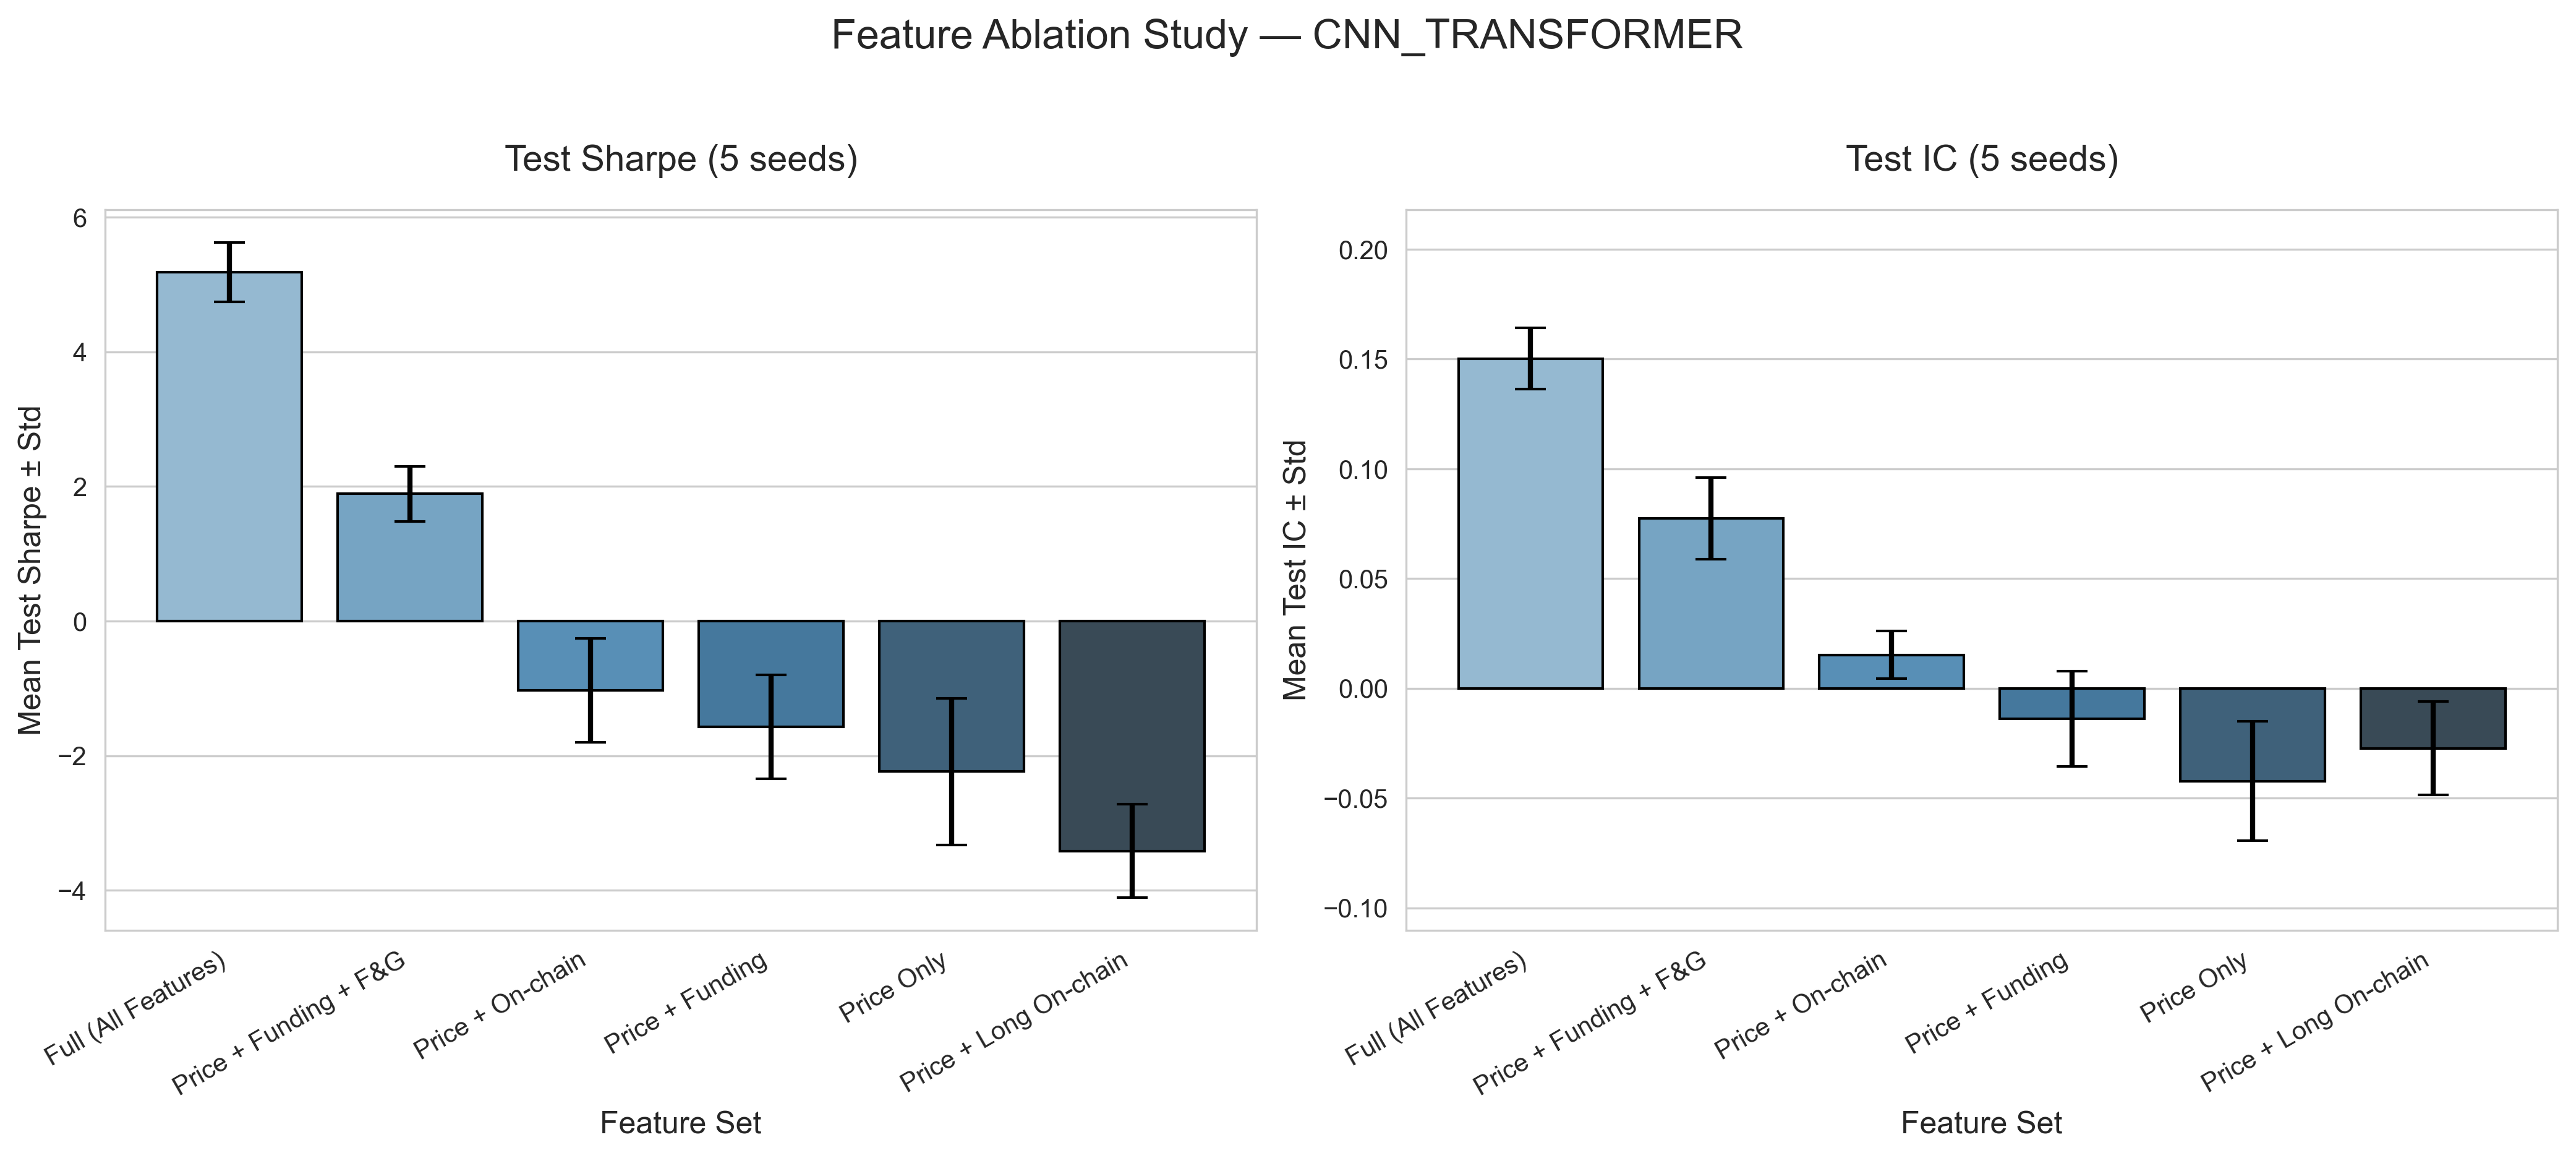
\includegraphics[width=0.80\textwidth]{../charts/feature_ablation_cnn_transformer.png}
\caption{CNN-Transformer在六种特征组合下的测试集夏普比率与IC对比（5种子均值$\pm$标准差）}
\label{fig:feature_ablation}
\end{figure}

\subsection{多种子稳定性分析}

为排除单一种子随机性对结论的影响，本文在5个不同随机种子（0, 1, 2, 42, 123）上重复了full特征集的全部实验。表\ref{tab:multi_seed}展示了跨种子统计。

\begin{table}[H]
\centering
\caption{full特征集上各模型跨5种子的测试集表现统计（均值$\pm$标准差）}
\label{tab:multi_seed}
\small
\begin{tabular}{lcccc}
\toprule
模型 & IC & Sharpe & MaxDD & AnnRet \\
\midrule
CNN-Transformer & 0.150$\pm$0.014 & 5.187$\pm$0.441 & 0.174$\pm$0.038 & 2.115$\pm$0.177 \\
Transformer & 0.129$\pm$0.008 & 3.531$\pm$0.903 & 0.198$\pm$0.021 & 1.446$\pm$0.367 \\
LSTM-Transformer & 0.125$\pm$0.015 & 3.016$\pm$1.855 & 0.253$\pm$0.144 & 1.234$\pm$0.759 \\
LSTM & 0.111$\pm$0.020 & 3.000$\pm$0.844 & 0.234$\pm$0.035 & 1.228$\pm$0.344 \\
PatchTST & 0.101$\pm$0.026 & 2.807$\pm$0.758 & 0.258$\pm$0.042 & 1.150$\pm$0.309 \\
XGBoost & 0.127$\pm$0.005 & 4.189$\pm$0.720 & 0.204$\pm$0.029 & 1.713$\pm$0.293 \\
TimeMixer & 0.103$\pm$0.018 & 3.480$\pm$1.131 & 0.218$\pm$0.067 & 1.424$\pm$0.463 \\
TCN & 0.069$\pm$0.039 & 0.616$\pm$1.966 & 0.386$\pm$0.218 & 0.252$\pm$0.807 \\
ModernTCN & 0.100$\pm$0.027 & 1.888$\pm$1.162 & 0.286$\pm$0.084 & 0.775$\pm$0.477 \\
DLinear & 0.074$\pm$0.016 & 0.368$\pm$0.632 & 0.378$\pm$0.071 & 0.151$\pm$0.259 \\
\bottomrule
\end{tabular}
\end{table}

从表\ref{tab:multi_seed}可以观察到：（1）CNN-Transformer稳健性最优（夏普标准差0.441，IC标准差0.014）。（2）部分模型种子敏感性高。LSTM-Transformer呈双峰分布（1/5种子崩溃至-0.25，其余4种子均值3.83）；TimeMixer跨种子夏普标准差1.13，主要波动来自seed=1（price\_funding\_fng上Sharpe=4.89但full上仅1.78）；TCN（标准差1.966）和ModernTCN（标准差1.162）波动剧烈。DLinear跨种子均值为所有模型最低（Sharpe=0.37），但标准差相对可控（0.63）。（3）链上协同效应跨种子稳健。CNN-Transformer的$\Delta$Sharpe在5种子间均为正值（+2.34至+4.22），跨种子均值+3.30$\pm$0.69。TimeMixer的$\Delta$Sharpe仅1/5种子为正值（+0.05），其余4种子均为负（范围$-$0.08至$-$3.11），均值$-$1.01——进一步确证多尺度时间维度混合无法替代跨特征源的显式建模。

\subsection{回测分析}

图\ref{fig:backtest1}展示了全部10个模型在full特征集测试集上的回测累计收益曲线。CNN-Transformer的回测曲线持续稳定上行（Sharpe=5.65，最大回撤仅18.6\%），XGBoost紧随其后（Sharpe=4.50，最大回撤18.3\%）；Transformer和PatchTST表现稳健（Sharpe 4.33/3.98）；LSTM-Transformer和LSTM虽有正收益但波动较大（最大回撤25.5\%/29.1\%）；TimeMixer取得中等正收益（Sharpe=1.78，最大回撤32.1\%）；ModernTCN和TCN几乎无盈利（Sharpe=0.17/0.05），前者在少数获利区间后迅速转为持续亏损（最大回撤41.5\%），与其训练集极端表现形成鲜明反差；DLinear全程亏损（Sharpe=-0.46，最大回撤49.0\%），确认线性模型在此多源异构、低信噪比场景下的局限。回测结果与表\ref{tab:full_results}的定量排名高度一致，进一步验证了三组架构分化的实际交易含义。

\begin{figure}[H]
\centering
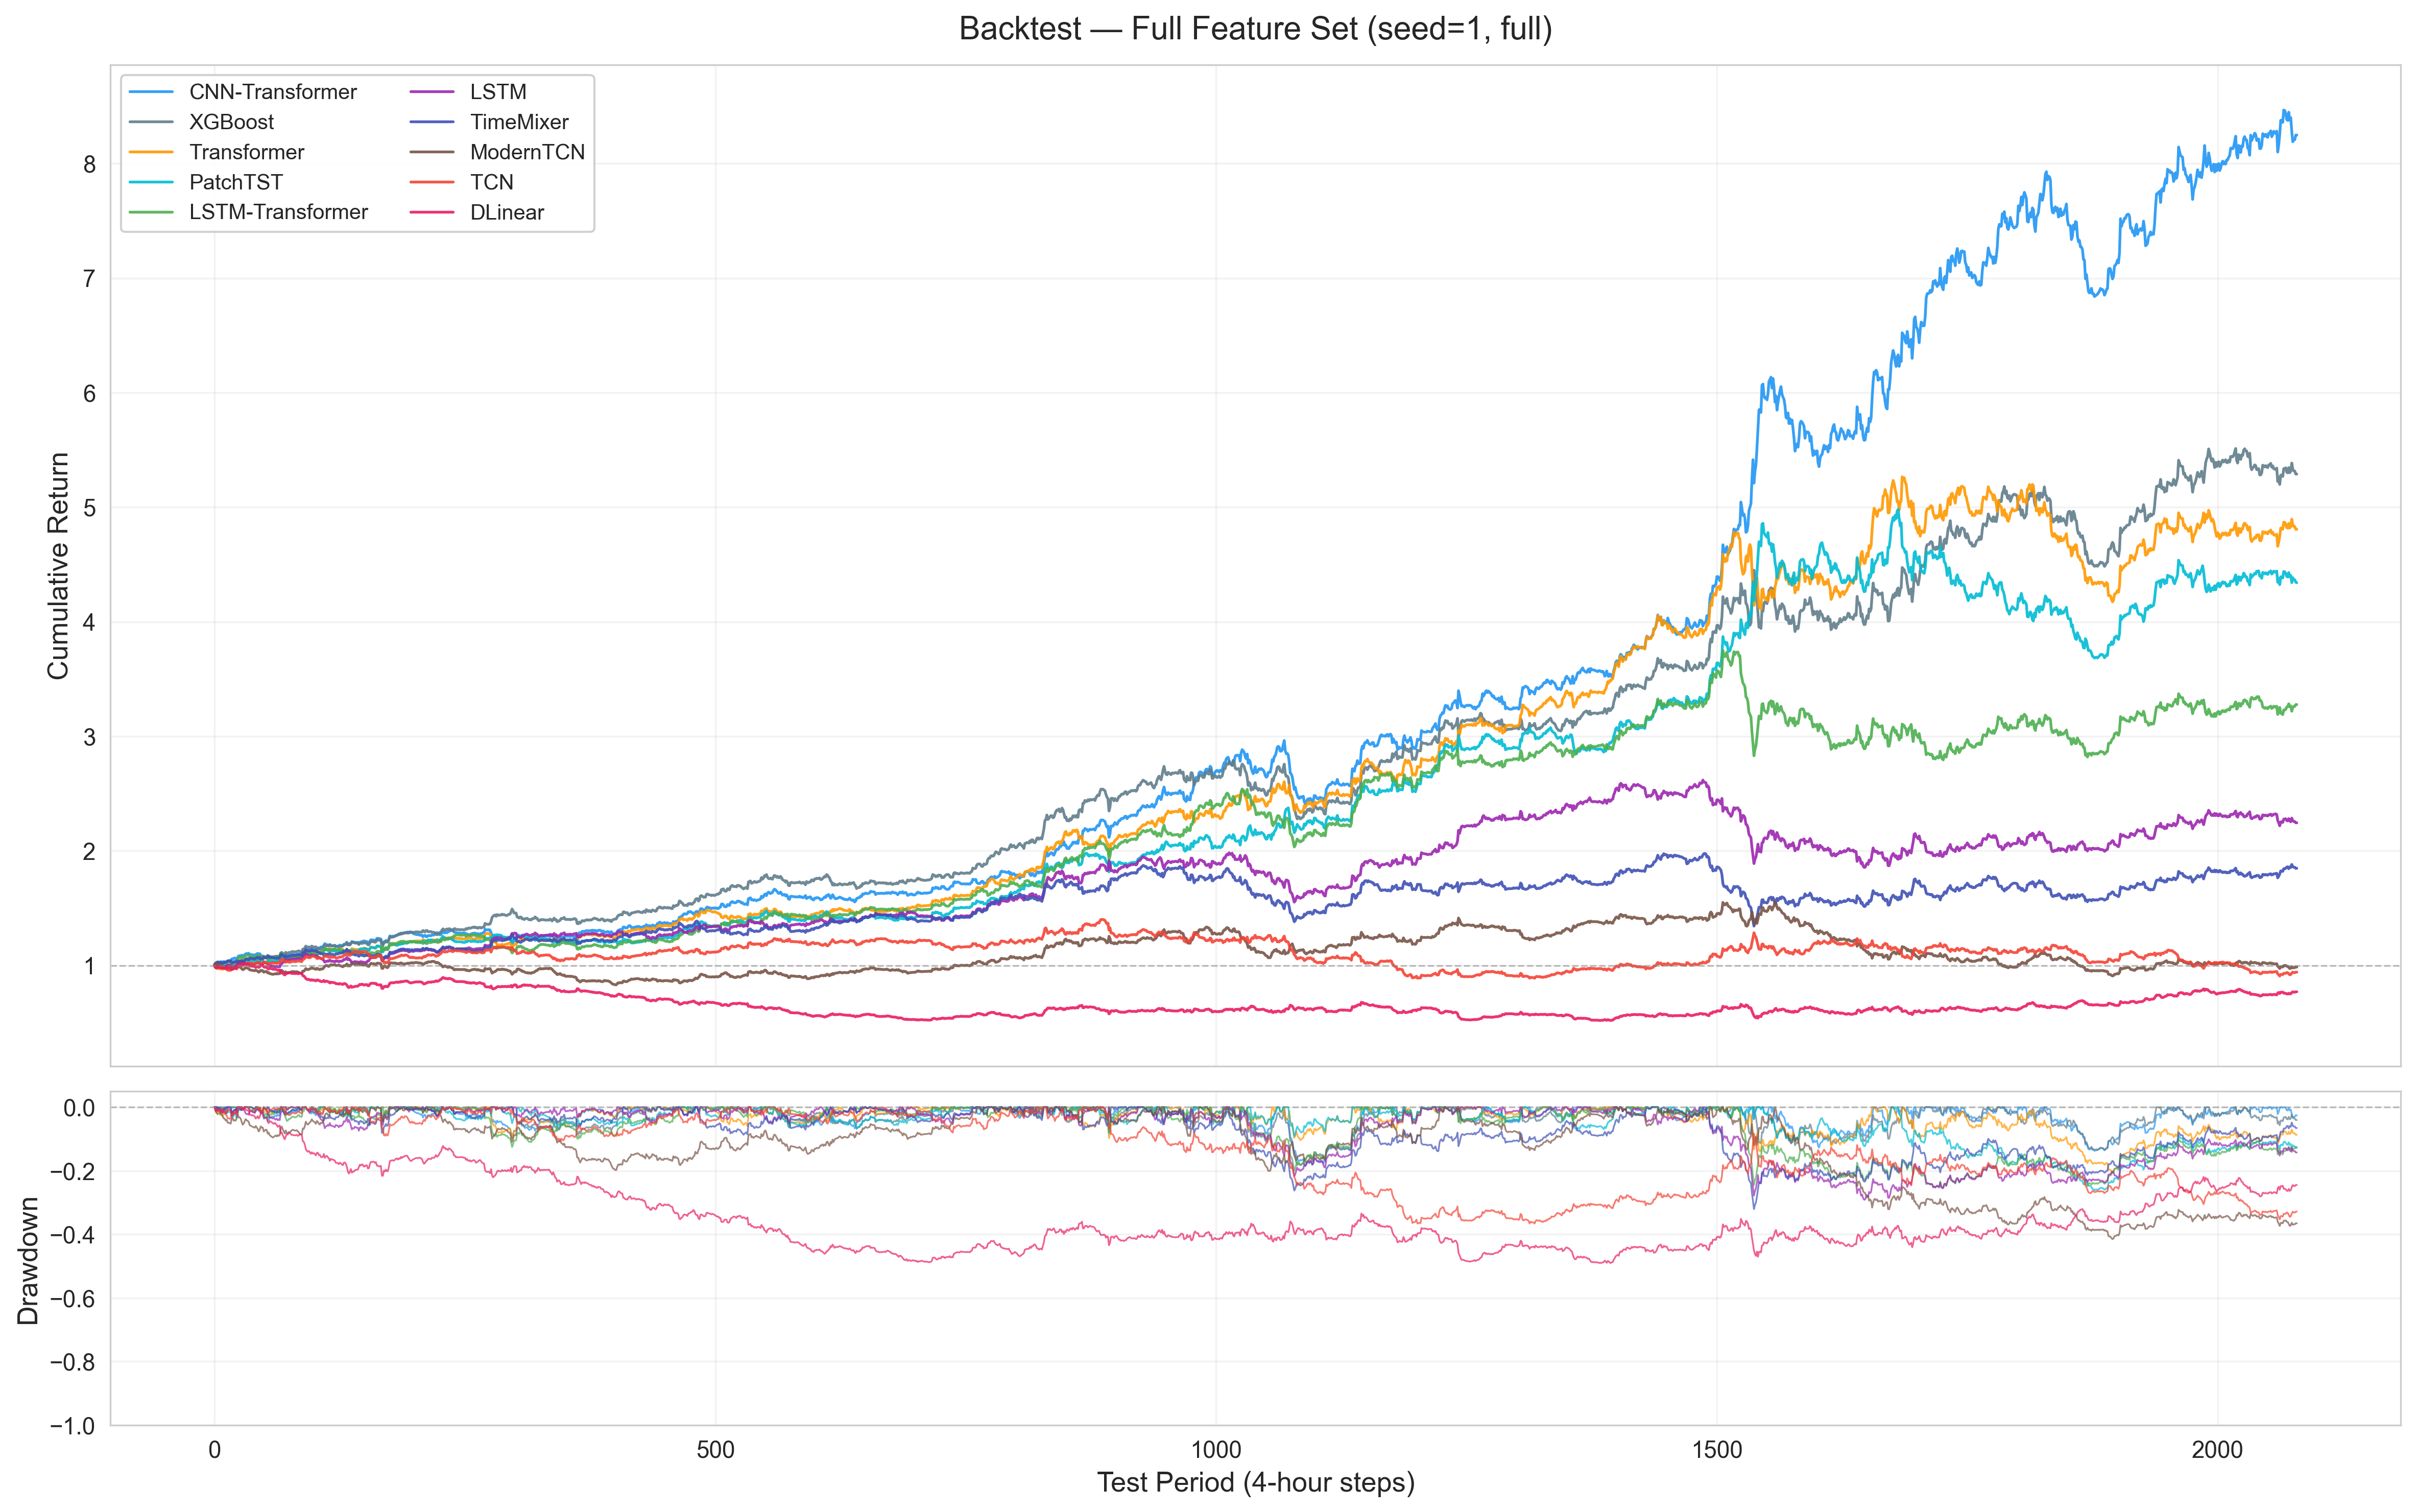
\includegraphics[width=0.88\textwidth]{../charts/backtest_full_all_models.png}
\caption{全部10个模型在full特征集上的回测累计收益曲线（seed=1）}
\label{fig:backtest1}
\end{figure}

\subsubsection{链上数据协同效应的回测可视化}

\newpage

图\ref{fig:backtest_synergy}展示了CNN-Transformer在full与price\_funding\_fng上的回测曲线对比，主要观察：

\begin{figure}[H]
\centering
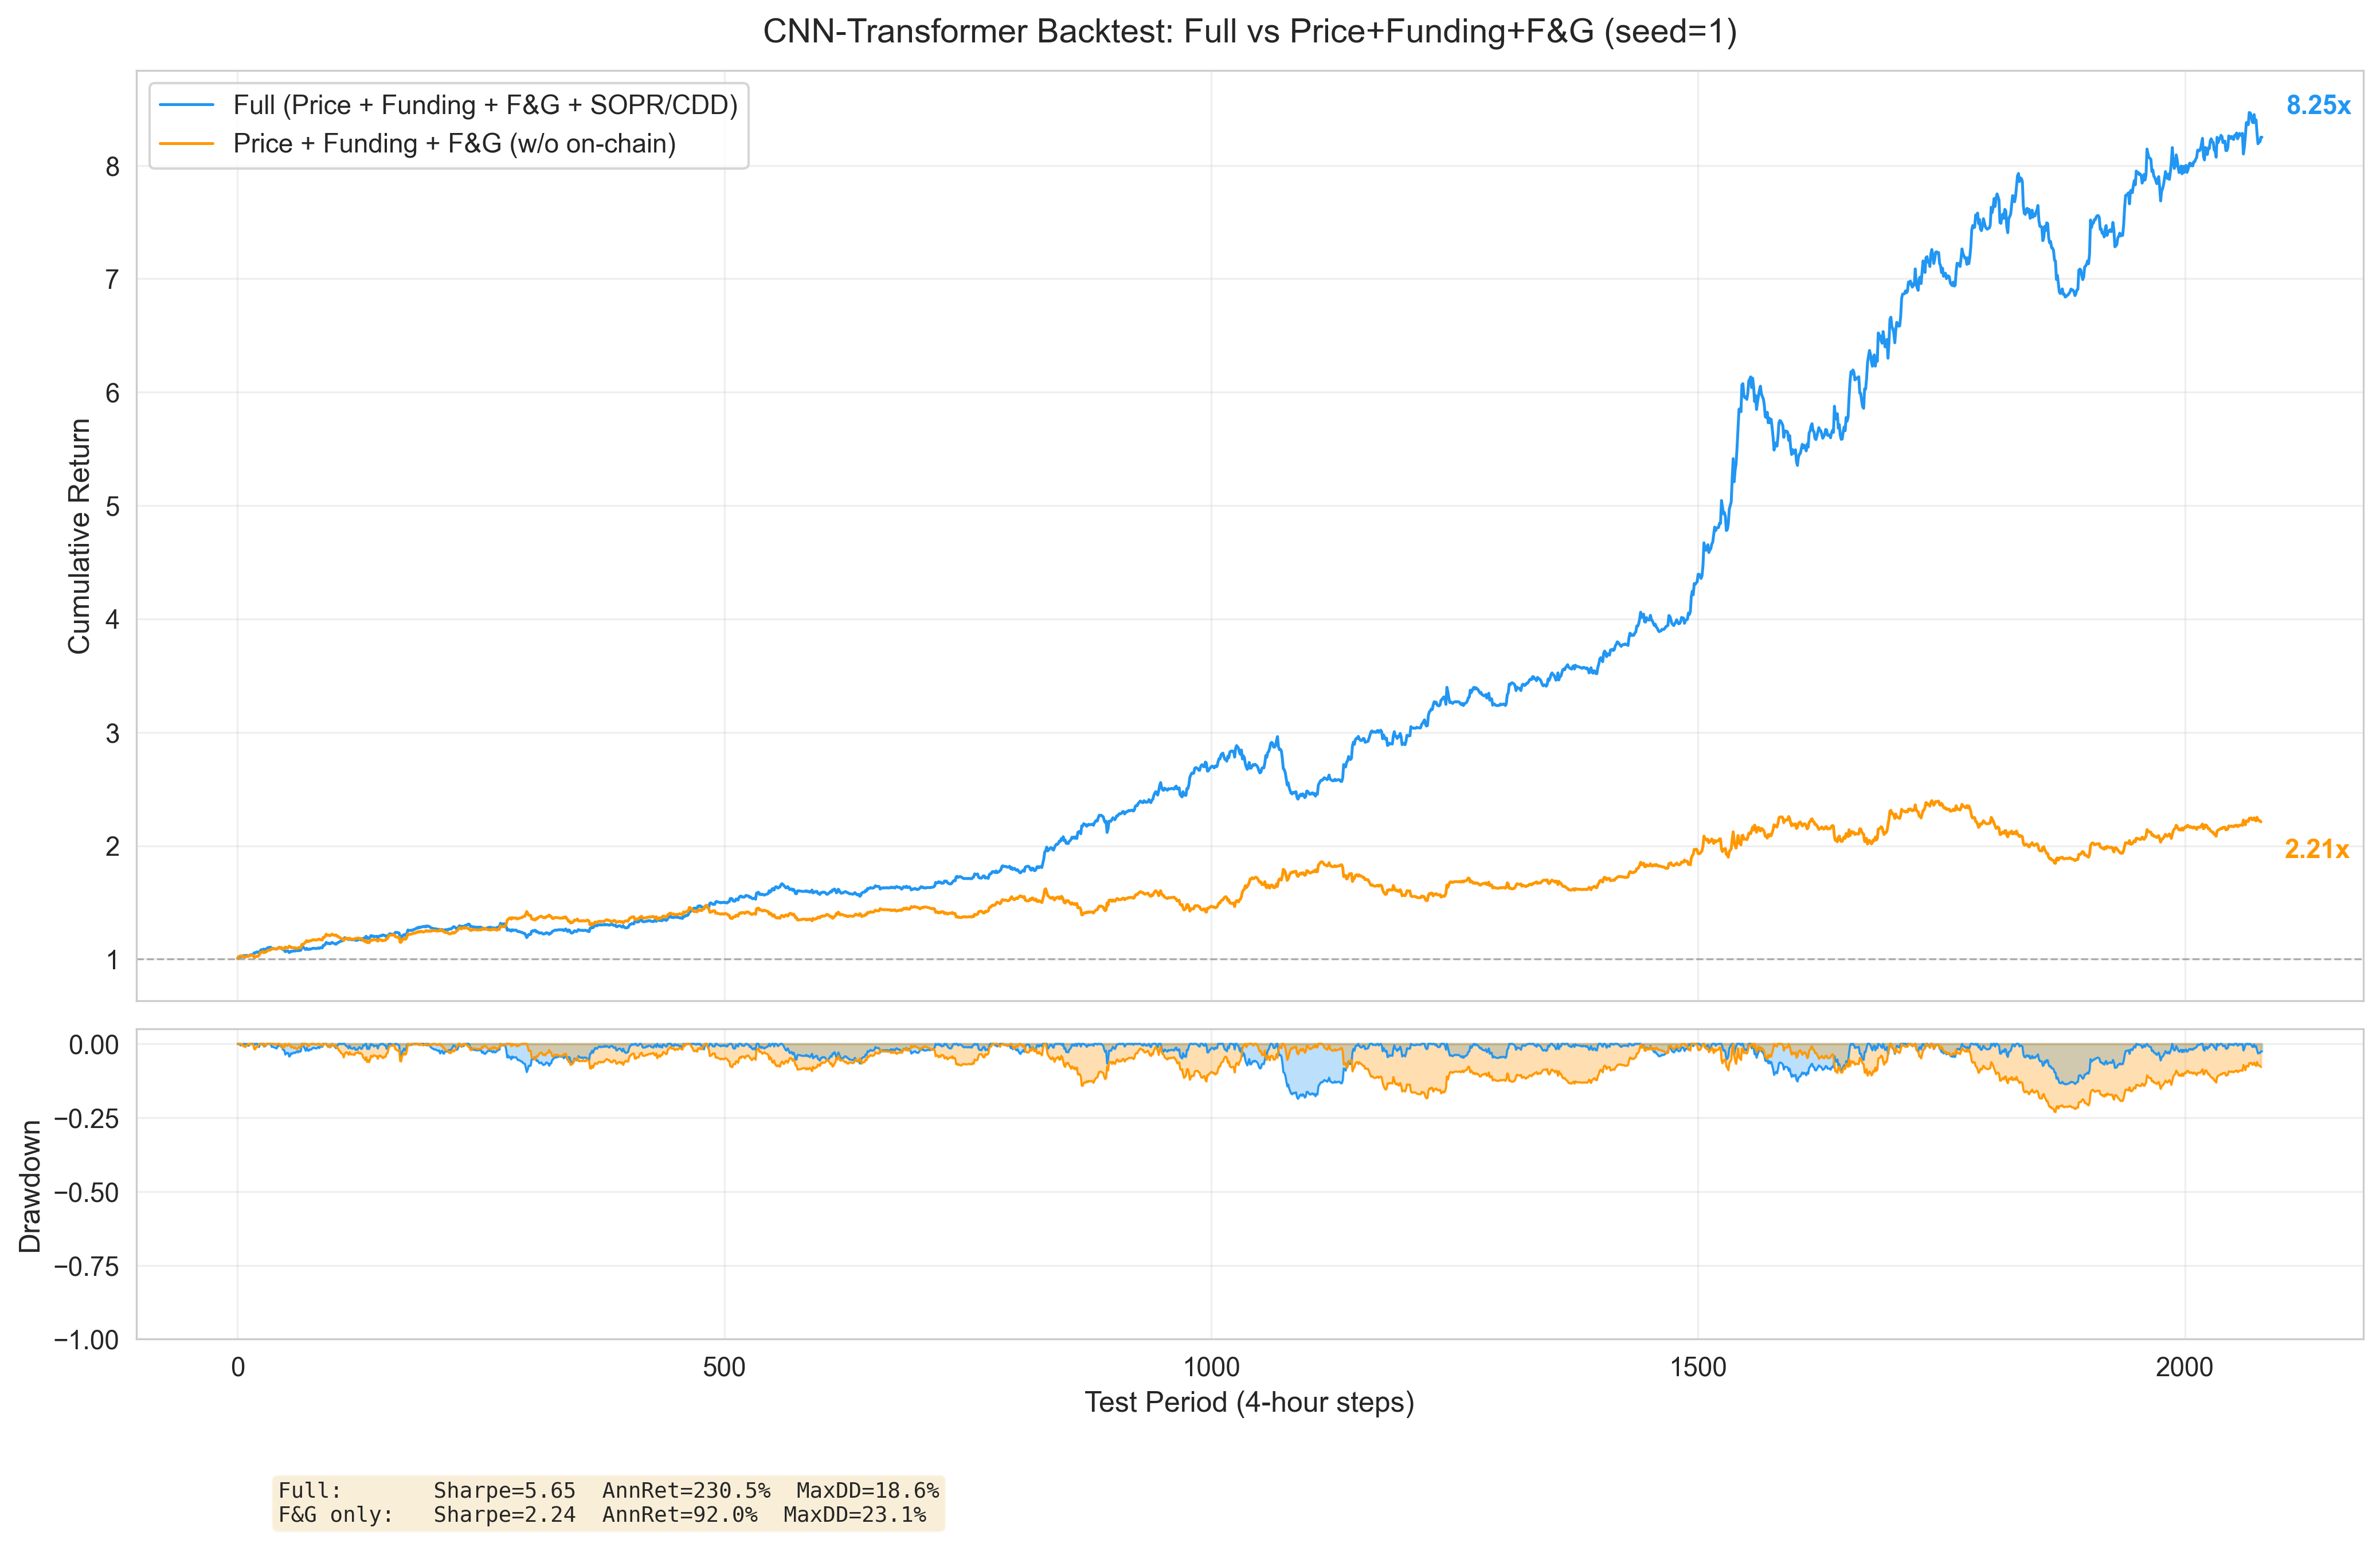
\includegraphics[width=0.88\textwidth]{../charts/backtest_synergy_full_vs_fng.png}
\caption{CNN-Transformer在full与price\_funding\_fng特征集上的回测对比（seed=1）：上图为累计收益曲线，下图为回撤曲线。full集（蓝）较fng集（橙）在Sharpe（5.65 vs 2.20）、年化收益（230.5\% vs 90.2\%）和最大回撤（18.6\% vs 23.1\%）三个维度上均实现全面提升}
\label{fig:backtest_synergy}
\end{figure}

\begin{itemize}[leftmargin=2.5em]
    \item full集与fng集的差距逐步扩大，测试最后full集累计收益（8.25$\times$）是fng集（2.21$\times$）的约3.7倍，与注意力机制逐步学习跨源组合的机制一致。
    \item full集最大回撤（18.6\%）显著低于fng集（23.1\%），SOPR和CDD提供的链上行为信息可能在极端市场条件下提前预警反转。
\end{itemize}

\subsection{统计显著性检验}

本文的核心论点是"链上数据的预测价值是条件性的且具有架构依赖性"，这需要从统计推断层面回答两个递进问题：（1）加入链上数据后，同一模型的预测误差是否显著降低？（2）不同架构间的性能差异是否统计可靠？为此，本节依次实施特征集DM检验（直接检验链上数据的增量贡献）、经济损失DM检验（策略层面验证）、模型间DM检验和Bootstrap检验（验证架构差异的显著性）。以下报告基于全部10个模型在full特征集上跨5种子平均预测的检验结果。

\subsubsection{特征集DM检验：链上数据是否降低了预测误差？}

为直接检验本文的核心论点，对全部10个模型分别实施成对特征集DM检验（full vs price\_funding\_fng，MSE损失）。负DM统计量表示full集（含SOPR/CDD链上数据）的MSE更低，即链上数据降低了预测误差。同时，还对price\_funding\_fng vs price\_funding（情绪贡献）和price\_funding vs price\_only（资金费率贡献）实施检验，以建立完整的特征消融统计证据链。结果见表\ref{tab:dm_feature_sets}和表\ref{tab:dm_feature_sets_full}。

% Feature-set DM tests — core thesis evidence
\begin{table}[ht]
\centering
\caption{特征集DM检验：链上数据（SOPR/CDD）对预测精度的增量贡献}
\label{tab:dm_feature_sets}
\footnotesize
\setlength{\tabcolsep}{2.5pt}
\resizebox{\textwidth}{!}{%
\begin{tabular}{lcccccc}
\toprule
模型 & 对比 & DM均值 & DM范围 & $p$均值 & 显著种子 & 结论 \\
\midrule
\bfseries CNN-Transformer & full vs price\_funding\_fng & \bfseries -2.46 & [-2.89, -2.05] & \bfseries 0.018 & 5/5 & \bfseries Significant (*) \\
Transformer & full vs price\_funding\_fng & -0.61 & [-1.65, +0.58] & 0.458 & 0/5 & Not sig. \\
LSTM-Transformer & full vs price\_funding\_fng & -1.66 & [-3.30, +0.33] & 0.329 & 3/5 & Not sig. \\
LSTM & full vs price\_funding\_fng & +0.92 & [-1.42, +3.39] & 0.261 & 1/5 & Not sig. \\
PatchTST & full vs price\_funding\_fng & -0.67 & [-2.47, +0.46] & 0.500 & 1/5 & Not sig. \\
XGBoost & full vs price\_funding\_fng & +1.41 & [-0.39, +3.57] & 0.374 & 2/5 & Not sig. \\
TCN & full vs price\_funding\_fng & +1.67 & [-0.29, +4.49] & 0.443 & 2/5 & Not sig. \\
ModernTCN & full vs price\_funding\_fng & +0.09 & [-0.87, +1.62] & 0.536 & 0/5 & Not sig. \\
DLinear & full vs price\_funding\_fng & +1.46 & [+0.41, +2.49] & 0.286 & 2/5 & Not sig. \\
TimeMixer & full vs price\_funding\_fng & +2.26 & [+0.76, +4.84] & 0.200 & 2/5 & Not sig. \\
\bottomrule
\multicolumn{7}{p{\textwidth}}{\scriptsize 注：** $p<0.01$, * $p<0.05$; 负DM统计量表示full集MSE低于price\_funding\_fng集（即链上数据降低了预测误差）。跨5种子（0,1,2,42,123）的成对DM检验。显著种子列表示达到$p<0.05$的种子数/有效种子总数。XGBoost仅price\_funding\_fng和full特征集有可用模型，其余特征集收敛失败。}
\end{tabular}%
}
\end{table}

% Full feature-set DM test matrix (all 3 comparisons)
\begin{table}[ht]
\centering
\caption{特征集消融DM检验：三组递进对比的完整结果}
\label{tab:dm_feature_sets_full}
\footnotesize
\setlength{\tabcolsep}{2.5pt}
\begin{tabular}{lccc}
\toprule
模型 & 链上协同 & 情绪贡献 & 资金费率贡献 \\
\midrule
CNN-Transformer & $-2.46^{*}$ & $-1.46$ & $-0.18$ \\
Transformer & $-0.61$ & $-1.79$ & $-0.41$ \\
LSTM-Transformer & $-1.66$ & $-2.33$ & $+0.42$ \\
LSTM & $+0.92$ & $-3.32$ & $+0.64$ \\
PatchTST & $-0.67$ & $-0.70$ & $+0.04$ \\
XGBoost & $+1.41$ & $-5.12^{**}$ & $+0.00$ \\
TCN & $+1.67$ & $-2.12$ & $-0.13$ \\
ModernTCN & $+0.09$ & $-1.15$ & $-0.83$ \\
DLinear & $+1.46$ & $-0.67$ & $-0.28$ \\
TimeMixer & $+2.26$ & $-4.03^{**}$ & $-0.06$ \\
\bottomrule
\multicolumn{4}{p{\textwidth}}{\footnotesize ** $p<0.01$, * $p<0.05$; 每格为DM统计量（跨5种子均值），负值表示更大特征集降低了MSE。}
\end{tabular}
\end{table}



从表\ref{tab:dm_feature_sets}可以得出以下核心发现：

（1）链上数据的有效性是架构条件性的，且仅有CNN-Transformer通过严格的跨种子显著性检验。在全部10个模型中，仅CNN-Transformer在5/5种子上均取得统计显著的MSE降低（跨种子DM=$-$2.46, $p=0.018$；逐种子DM范围[$-$2.89, $-$2.05]，全部$p<0.05$）。LSTM-Transformer在3/5种子上取得正向效果但跨种子未达一致性显著（DM=$-$1.66, $p=0.33$）。其余8个模型——包括ICLR 2024 SOTA TimeMixer（DM=+2.26）——的full集MSE均不显著低于或不高于price\_funding\_fng集。这一结果从预测精度维度直接回答了论文的核心问题：链上数据并非普遍有效，其预测价值严格依赖于模型架构是否具备层级化跨源特征处理能力。

（2）情绪特征（恐慌贪婪指数）的贡献最为普适且显著。price\_funding\_fng vs price\_funding的DM检验显示：XGBoost（DM=$-$5.12, $p<0.001$, 5/5种子显著）、TimeMixer（DM=$-$4.03, $p=0.002$, 5/5种子显著）、LSTM（DM=$-$3.32, $p=0.054$, 4/5显著）和LSTM-Transformer（DM=$-$2.33, 3/5显著）均从情绪特征中获得统计显著的MSE改善。情绪信号在加密货币短期预测中的价值具有跨架构的普适性。

（3）资金费率的独立贡献弱且不一致。price\_funding vs price\_only的DM检验中，Transformer是唯一在多数种子上取得显著改善的模型（3/5种子，DM=$-$0.41, $p=0.070$），其余模型的MSE变化大多不显著。资金费率信号在4小时频率上的独立预测信息有限，其价值主要通过与情绪和链上信号的联合发挥作用。

（4）特征集DM检验与策略夏普协同效应形成交叉验证。表\ref{tab:dm_feature_sets_full}的三组递进对比揭示了清晰的层级结构：情绪特征对多数模型有益（普适层），链上特征仅对混合架构有益（条件层），资金费率贡献有限且依赖架构（弱信号层）。这与第6.2节中$\Delta$Sharpe的三组分化结论高度一致——CNN-Transformer在MSE和Sharpe两个维度均保持一致的链上协同增益，提供了预测精度与策略表现的双重统计支撑。

\subsubsection{基于经济损失函数的DM检验}

上述特征集DM检验从预测精度维度确认了链上数据的条件有效性，本节从策略收益维度提供互补证据。鉴于MSE量级极小（$10^{-4}$）严重压缩了模型间差异，以策略收益的负值作为经济损失函数实施DM检验，负DM统计量表示行模型策略收益更优。表\ref{tab:dm_econ}展示了以CNN-Transformer为基准的逐种子DM检验结果及跨种子胜率统计。

% Economic loss DM test (Chinese)
\begin{table}[ht]
\centering
\caption{基于策略收益的DM检验（CNN-Transformer为行模型基准，full特征集）}
\label{tab:dm_econ}
\small
\begin{tabular}{lccccc}
\toprule
对比模型 & 胜出种子 & DM均值 & DM范围 & 显著种子 & 结论 \\
\midrule
vs Transformer & 4/5 & $-2.60$ & [$-4.75$, $+0.98$] & 3/5 & 一致更优 \\
vs LSTM-Transformer & 3/5 & $+0.14$ & [$-0.53$, $+1.03$] & 0/5 & 边际混合 \\
vs LSTM & 4/5 & $-1.10$ & [$-3.52$, $+0.36$] & 1/5 & 一致更优 \\
vs PatchTST & 4/5 & $-1.47$ & [$-4.73$, $+0.26$] & 1/5 & 一致更优 \\
vs XGBoost & 3/5 & $+0.23$ & [$-0.64$, $+1.50$] & 0/5 & 边际混合 \\
vs TCN & 5/5 & $-3.18$ & [$-4.10$, $-1.33$] & 4/5 & 一致且显著更优 \\
vs ModernTCN & 5/5 & $-2.05$ & [$-3.55$, $-0.32$] & 2/5 & 一致更优 \\
vs DLinear & 5/5 & $-4.70$ & [$-6.68$, $-2.77$] & 5/5 & 一致且显著更优 \\
vs TimeMixer & 3/5 & $-0.59$ & [$-1.80$, $+0.25$] & 0/5 & 边际混合 \\
\bottomrule
\multicolumn{6}{p{\textwidth}}{\small 胜出种子 = CNN-Transformer优于对比模型的种子数（共5种子）；负DM = CNN-Transformer策略收益更高。显著种子 = $p<0.05$的种子数。} \\
\end{tabular}
\end{table}


CNN-Transformer在全部9个对比模型上于多数种子中取得更高策略收益，对TCN、ModernTCN和DLinear的优势在多数种子上显著。DLinear在全部5个种子上均被显著超越（DM=$-$4.70, 5/5种子$p<0.01$），而与Transformer、LSTM-Transformer和TimeMixer的差异部分依赖于种子。8/9模型的DM均值为负这一广泛一致的方向性进一步确认：MSE空间掩盖了策略相关的性能差距，这些差距在经济损失空间中变得清晰可见。

\subsubsection{模型间DM检验}

上述两组检验直接验证了本文的核心论点（链上数据的条件有效性及其架构依赖性）。作为补充，本节提供模型间的成对DM检验\cite{diebold1995}（MSE损失），以评估不同架构间预测精度差异的统计可靠性。表\ref{tab:dm_mse}展示了10个模型的完整成对DM检验结果。CNN-Transformer的MSE显著低于除Transformer外的所有模型（$p<0.05$），与Transformer差异不显著（$p=0.619$）。DLinear的MSE显著高于CNN-Transformer和Transformer，TimeMixer的MSE介于纯注意力和纯卷积之间，与ModernTCN差异不显著（$p=0.142$）。需注意MSE量级极小（$10^{-4}$），纯误差指标下模型差异被严重压缩——这也是为何前文优先使用特征集DM和经济损失DM来检验核心论点。

% DM Test (MSE loss) — Upper triangle
\begin{table}[ht]
\centering
\caption{Diebold-Mariano检验结果（MSE损失）——上三角为DM统计量及p值}
\label{tab:dm_mse}
\footnotesize
\setlength{\tabcolsep}{1.5pt}
\resizebox{\textwidth}{!}{%
\begin{tabular}{lcccccccccc}
\toprule
 & \multicolumn{1}{c}{CNN-Tr.} & \multicolumn{1}{c}{Tr.} & \multicolumn{1}{c}{LSTM-Tr.} & \multicolumn{1}{c}{LSTM} & \multicolumn{1}{c}{PatchTST} & \multicolumn{1}{c}{XGBoost} & \multicolumn{1}{c}{TCN} & \multicolumn{1}{c}{M.TCN} & \multicolumn{1}{c}{DLinear} & \multicolumn{1}{c}{T.Mixer} \\
\midrule
CNN-Tr. & -- & +0.50 (.619) & $-$3.81 (.000) ** & $-$3.07 (.002) ** & $-$2.41 (.016) * & $-$3.78 (.000) ** & $-$4.21 (.000) ** & $-$2.21 (.027) * & $-$2.70 (.007) ** & $-$3.37 (.001) ** \\
Tr. & -- & -- & $-$3.60 (.000) ** & $-$2.87 (.004) ** & $-$2.43 (.015) * & $-$3.62 (.000) ** & $-$3.73 (.000) ** & $-$2.20 (.028) * & $-$2.91 (.004) ** & $-$3.10 (.002) ** \\
LSTM-Tr. & -- & -- & -- & +3.58 (.000) ** & +2.89 (.004) ** & +0.06 (.956) & +0.42 (.674) & +2.73 (.006) ** & +0.04 (.966) & +2.47 (.014) * \\
LSTM & -- & -- & -- & -- & +1.11 (.267) & $-$3.08 (.002) ** & $-$2.00 (.045) * & +1.14 (.253) & $-$1.04 (.300) & $-$0.40 (.687) \\
PatchTST & -- & -- & -- & -- & -- & $-$2.77 (.006) ** & $-$2.46 (.014) * & +0.17 (.862) & $-$1.55 (.120) & $-$1.27 (.205) \\
XGBoost & -- & -- & -- & -- & -- & -- & +0.41 (.682) & +2.68 (.007) ** & +0.03 (.973) & +2.12 (.034) * \\
TCN & -- & -- & -- & -- & -- & -- & -- & +2.74 (.006) ** & $-$0.15 (.878) & +1.64 (.100) \\
M.TCN & -- & -- & -- & -- & -- & -- & -- & -- & $-$1.60 (.109) & $-$1.47 (.142) \\
DLinear & -- & -- & -- & -- & -- & -- & -- & -- & -- & +0.86 (.392) \\
T.Mixer & -- & -- & -- & -- & -- & -- & -- & -- & -- & -- \\
\bottomrule
\multicolumn{11}{p{\textwidth}}{\scriptsize 注：下三角为对称值；括号内为$p$值；** $p<0.01$, * $p<0.05$; 基于跨种子平均预测的MSE损失计算。CNN-Tr.=CNN-Transformer, Tr.=Transformer, LSTM-Tr.=LSTM-Transformer, M.TCN=ModernTCN, T.Mixer=TimeMixer。}
\end{tabular}%
}
\end{table}

% Bootstrap Sharpe Ratio Difference Test
\begin{table}[ht]
\centering
\caption{Bootstrap夏普比率差异检验（Ledoit \& Wolf, 2008）}
\label{tab:bootstrap_sharpe}
\footnotesize
\setlength{\tabcolsep}{2.5pt}
\resizebox{\textwidth}{!}{%
\begin{tabular}{llrrcl}
\toprule
模型A & 模型B & $\Delta$Sharpe & 95\% CI & $p$值 & 显著性 \\
\midrule
CNN-Transformer & Transformer & +0.8926 & [-0.5276, +2.3031] & 0.2180 & -- \\
CNN-Transformer & LSTM-Transformer & +1.4825 & [-0.0041, +2.9958] & 0.0526 & -- \\
CNN-Transformer & LSTM & +1.2657 & [-0.3558, +2.9551] & 0.1289 & -- \\
CNN-Transformer & PatchTST & +2.1705 & [+0.7180, +3.6442] & 0.0029 & ** \\
CNN-Transformer & XGBoost & +1.5091 & [-0.1505, +3.1752] & 0.0761 & -- \\
CNN-Transformer & TCN & +5.0367 & [+3.1892, +6.9323] & 0.0000 & ** \\
CNN-Transformer & ModernTCN & +3.2297 & [+1.4927, +4.9520] & 0.0001 & ** \\
CNN-Transformer & DLinear & +5.5540 & [+3.2544, +7.8952] & 0.0000 & ** \\
CNN-Transformer & TimeMixer & +1.1349 & [-0.3535, +2.6399] & 0.1418 & -- \\
\bottomrule
\multicolumn{6}{p{\textwidth}}{\scriptsize 注：** $p<0.01$, * $p<0.05$; 正$\Delta$Sharpe表示模型A优于模型B; 10,000次Bootstrap; 基于跨种子平均收益计算。}
\end{tabular}%
}
\end{table}



\subsubsection{Bootstrap夏普比率差异检验}

鉴于加密货币收益预测的最终目标是策略表现而非预测精度，本文进一步采用Ledoit和Wolf（2008）的Bootstrap方法\cite{ledoit2008}检验模型间夏普比率差异的显著性。与DM检验一致，先对跨种子策略收益在时间点层面取平均，再基于10,000次Bootstrap重采样构建学生化置信区间并计算$p$值。表\ref{tab:bootstrap_sharpe}展示了以CNN-Transformer为基准的全部成对检验结果。

CNN-Transformer的夏普比率在$p<0.01$水平上显著优于PatchTST、TCN、ModernTCN和DLinear，与Transformer、LSTM、LSTM-Transformer、XGBoost和TimeMixer的差异未达5\%显著性水平（$p=0.053$--0.218）。DLinear的夏普显著低于所有深度模型（vs CNN-Transformer $p=0.0000$，vs TimeMixer $p=0.0005$），确认线性分解在此场景下的局限。TimeMixer与CNN-Transformer差异不显著（$\Delta$Sharpe=+1.13, $p=0.14$），表明其多尺度混合机制在跨种子平均后具有一定竞争力，但其高种子敏感性（标准差1.13）削弱了统计推断力。值得注意的是，$\Delta$Sharpe在协同利用组一致为正（$>+2$）、在负向干扰组一致为负（$<-1.5$），所有5种子呈现一致的符号模式，与特征集DM检验的结论相互印证。

\subsection{滑动窗口验证实验}

上述实验均基于单一的时序划分（训练集2020--2024、验证集2024--2025、测试集2025--2026），模型在测试集上的优异表现是否具备跨时间窗口的鲁棒性仍待检验，这也是时序预测评估中常被忽视的关键维度\cite{cerqueira2020}。为此，本文引入滑动窗口验证：将全数据集划分为8个固定大小的滑动窗口，每个窗口训练2年（约4,380条序列）并在随后6个月（约1,095条序列）上进行测试，窗口滑动步长为6个月。该设计覆盖2022年上半年至2025年下半年的不同市场体制（熊市、反弹、牛市、震荡），评估模型表现的跨窗口均值、标准差与极端值，以补充单窗口评估无法提供的体制依赖信息。

\input{../results/sliding_window.tex}

\begin{figure}[ht]
\centering
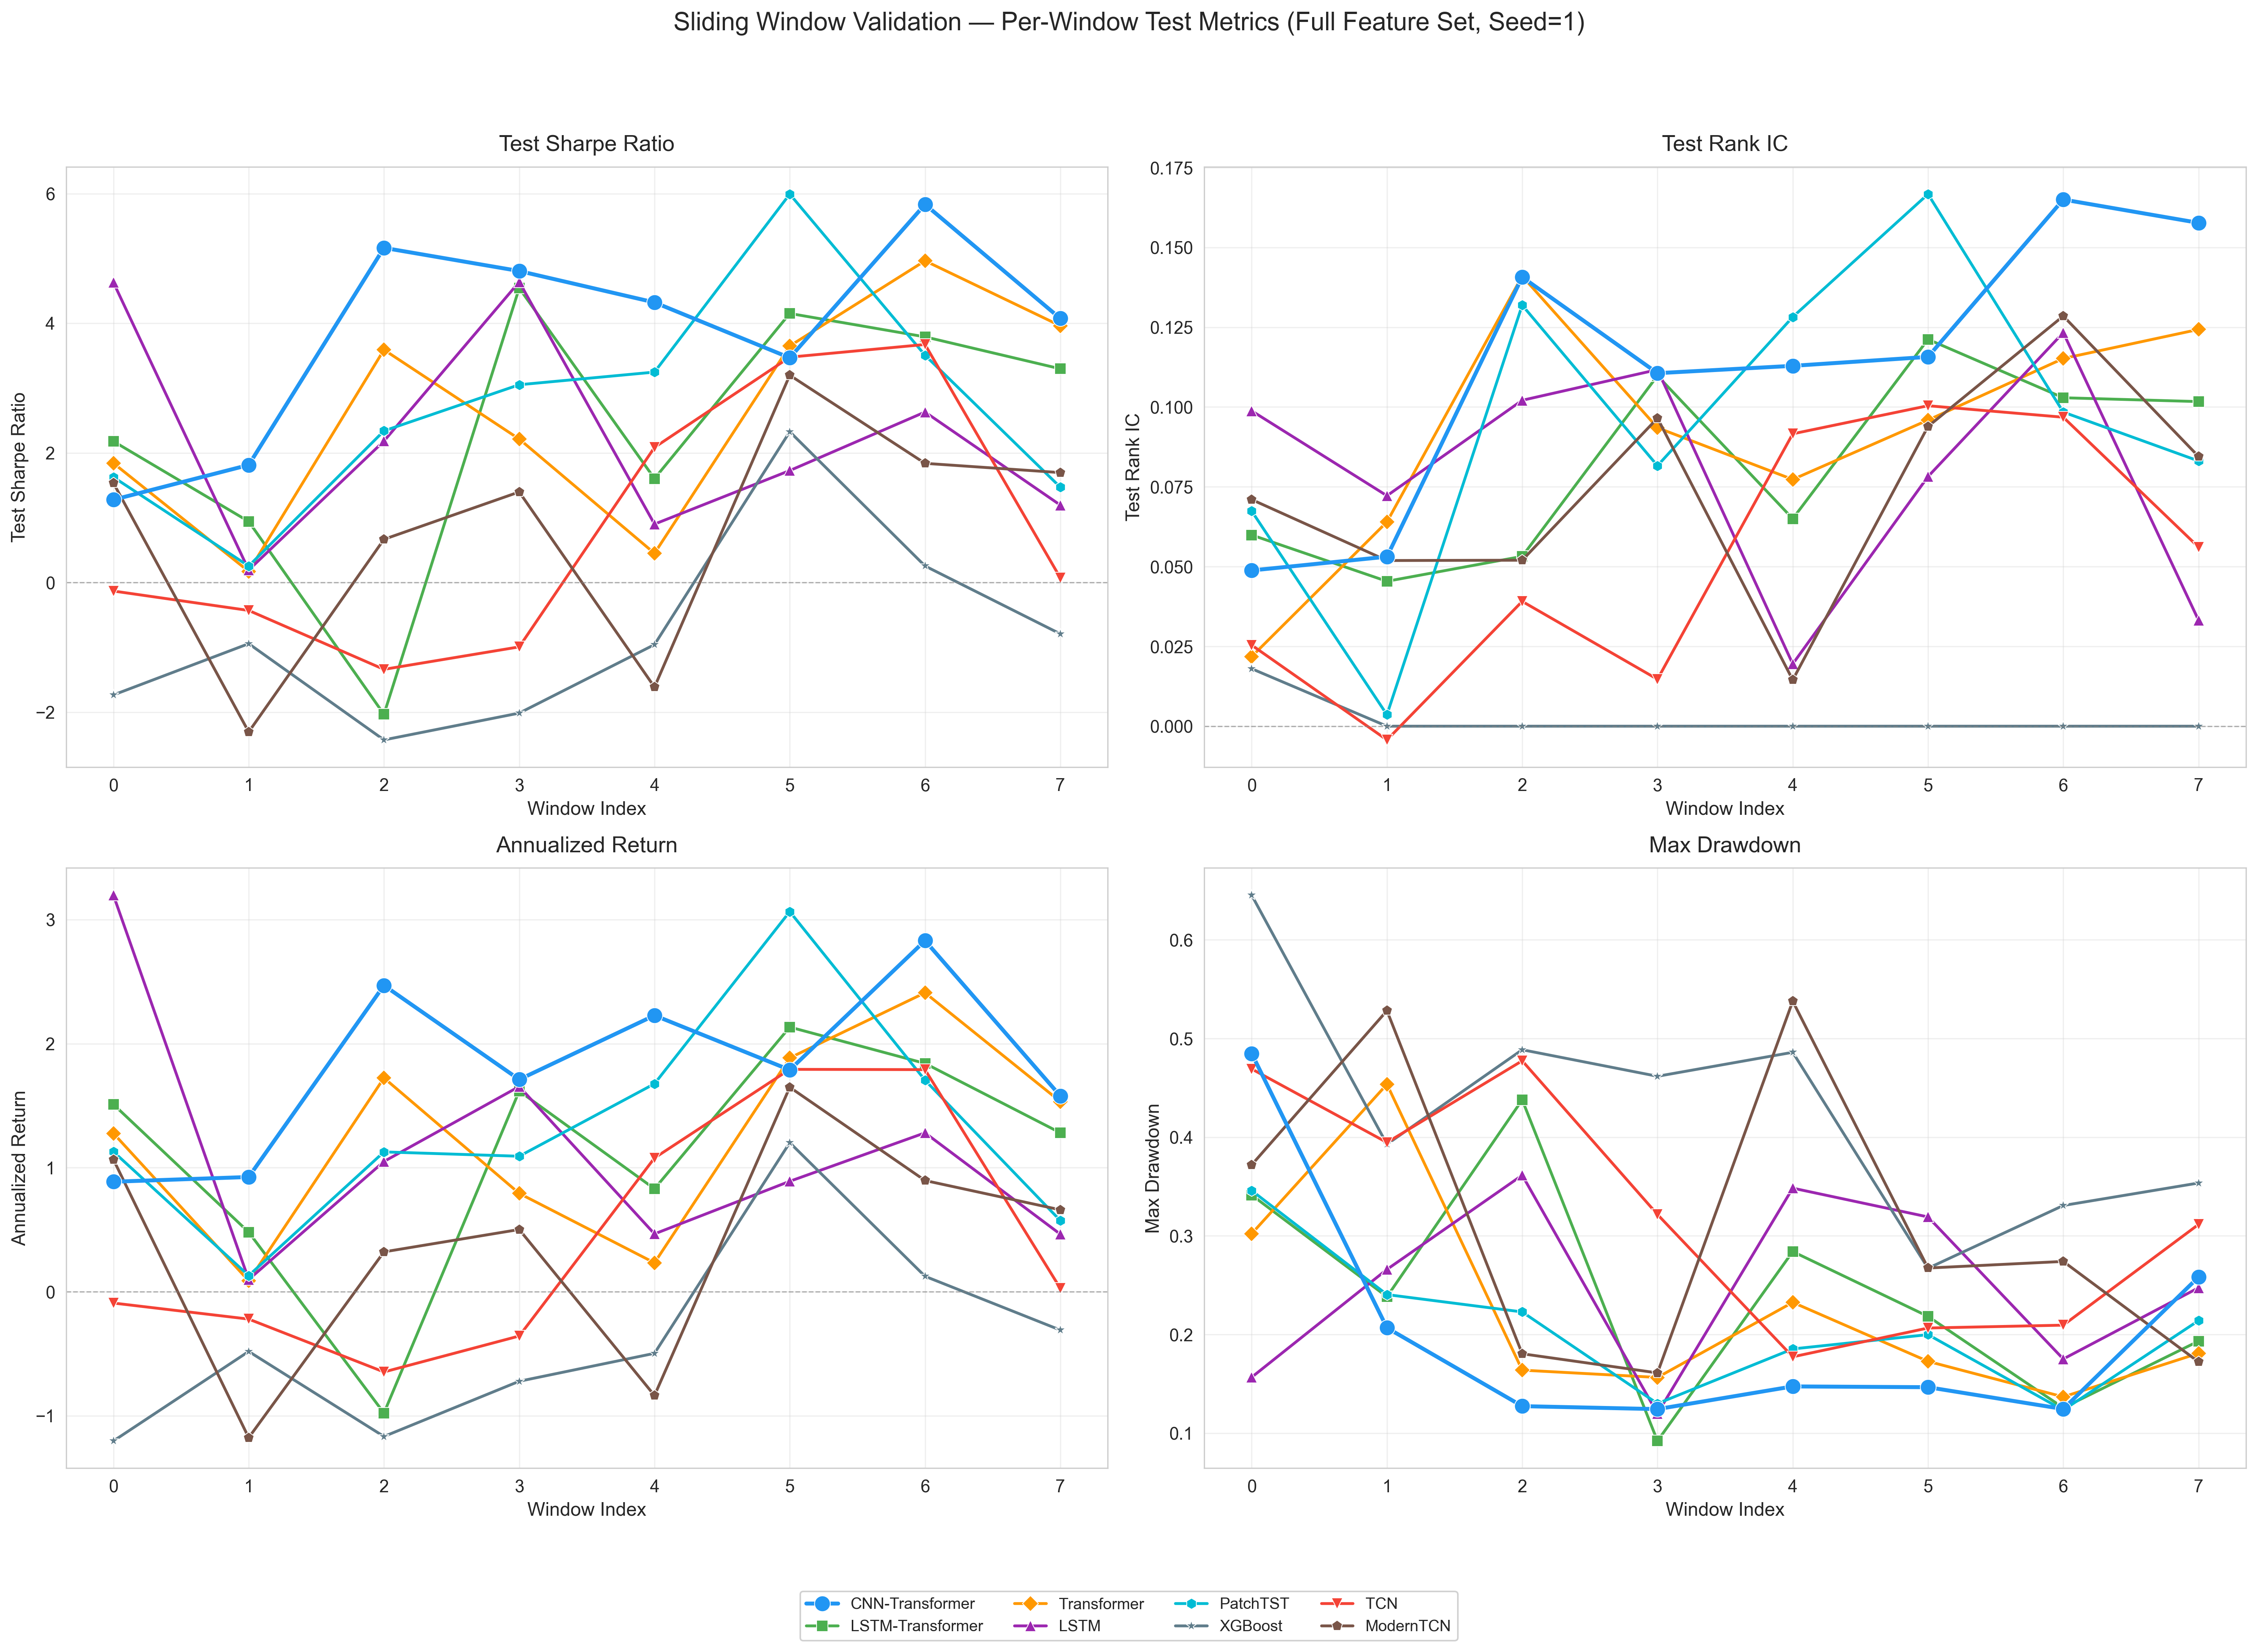
\includegraphics[width=0.95\textwidth]{../charts/sliding_window_metrics.png}
\caption{滑动窗口验证：各模型在full特征集上的测试夏普比率、IC、年化收益和最大回撤随窗口的变化（seed=1）。窗口0--7依次覆盖2022 H1至2025 H2，涵盖熊市、反弹、牛市、震荡等不同市场体制}
\label{fig:sliding_window_metrics}
\end{figure}

表\ref{tab:sliding_window}和图\ref{fig:sliding_window_metrics}展示了全部10个模型在8个时间窗口上的测试表现，主要发现如下：

（1）CNN-Transformer是全窗口表现最优的模型，TimeMixer紧随其后排名第二。4个模型（CNN-Transformer、PatchTST、Transformer、LSTM）在全部8个窗口中保持正夏普，TimeMixer（7/8窗口为正，仅W1=$-$0.01）和LSTM-Transformer（7/8窗口为正，仅W2=$-$2.03）各有1个窗口为负但跨窗口均值仍为正。CNN-Transformer跨窗口均值3.85（标准差1.59），最低W0=1.28，最高W6=5.83。TimeMixer以均值3.19（标准差1.51）位居第二，表明其多尺度时序混合机制虽不能利用链上数据（第6.2节），但在动态市场体制中仍保持稳健的预测力。

（2）滑动窗口揭示了比静态评估更丰富的架构层次。跨窗口均值：CNN-Transformer（3.85）$>$ TimeMixer（3.19）$\gg$ PatchTST（2.69）$\approx$ Transformer（2.61）$\approx$ LSTM-Transformer（2.31）$\approx$ LSTM（2.26）$\gg$ ModernTCN（0.80）$\approx$ TCN（0.80）$\gg$ XGBoost（$-0.79$）$\approx$ DLinear（$-1.26$）。XGBoost静态高夏普（4.50）在滑动窗口下完全消失（均值$-0.79$），DLinear跨窗口均值$-1.26$（标准差2.15）确认线性模型在各市场体制下的结构性不足，其在W1极端崩溃至$-5.38$。

（3）ModernTCN和TCN严重过拟合，DLinear跨窗口波动极端。ModernTCN在全部8个窗口的训练集夏普均超32，测试集均值仅0.80。DLinear跨窗口标准差高达2.15，在W0和W6取得正值（0.53、0.80），但在W1崩溃至$-5.38$，暴露出线性模型在不同市场体制间的高度不稳定性。链上协同效应的发挥存在"市场体制下限条件"——熊市窗口中衍生品和情绪信号弱化时，链上数据的增量价值被压缩。


\subsection{讨论}

以下从四个维度对实验结果进行延伸讨论：

\begin{enumerate}[label=(\arabic*),leftmargin=2.5em]
    \item \textbf{链上数据条件有效性的机制解释。}SOPR和CDD反映已发生的链上行为，属于"慢变量"，需通过衍生品博弈和市场情绪来"激活"——单独看SOPR$<1$是模糊信号，但与极端恐惧（FNG$<25$）和负资金费率同时出现时，三信号汇合使"恐慌性底部"概率大幅上升。混合架构的层级化管线（CNN局部特征提取$\to$Transformer全局交互）恰好适配此类多源联合分布的捕获：卷积层在局部感受野内压缩时序模式，Transformer的自注意力机制跨时间步建模特征间的高阶交互。这一机制解释了三组分类的存在性——纯循环/纯卷积架构缺乏全局跨特征交互能力，错过跨源协同信号；多尺度混合架构（TimeMixer）的PDM模块在分解后独立处理各尺度，可能破坏了跨源特征的联合分布结构。

    \item \textbf{关于指标绝对水平的审慎解读。}本文最优模型测试夏普跨5种子均值5.19、年化收益211.5\%，应视为实验设定下的上限估计：（1）策略未考虑保证金和仓位约束；（2）仅扣除5 bps双边手续费，实际摩擦成本可达20--50 bps；（3）数据区间覆盖BTC牛市周期；（4）年化公式（$\times 2190$周期）放大单期优势。模型间的相对排名及协同效应的跨架构一致性才是可迁移的核心结论。建议后续研究采用多种子滑动窗口下的夏普均值（如协同利用组跨窗口均值3.85）作为更审慎的性能基准。

    \item \textbf{交易成本与换手率：从预测到部署的现实约束。}图\ref{fig:cost_sensitivity}和表\ref{tab:cost_sensitivity}展示了0--50 bps范围内的成本敏感性分析：

    % Auto-generated cost sensitivity LaTeX table
\begin{table}[ht]
\centering
\caption{Transaction cost sensitivity analysis --- strategy performance across fee levels (cross-seed average)}
\label{tab:cost_sensitivity}
\footnotesize
\setlength{\tabcolsep}{4pt}
\resizebox{\textwidth}{!}{%
\begin{tabular}{lcccccc}
\toprule
Fee & CNN-Transformer & Transformer & LSTM-Transformer & XGBoost & DLinear & TimeMixer \\
\midrule
0 bps & 6.82 / 277\% / 14\% & 5.77 / 235\% / 15\% & 5.26 / 215\% / 15\% & 4.90 / 200\% / 17\% & 3.26 / 134\% / 28\% & 4.74 / 194\% / 15\% \\
5 bps & 6.09 / 248\% / 15\% & 4.70 / 192\% / 17\% & 4.70 / 192\% / 16\% & 4.50 / 184\% / 18\% & 0.93 / 38\% / 40\% & 4.18 / 171\% / 17\% \\
10 bps & 5.36 / 218\% / 16\% & 3.63 / 149\% / 18\% & 4.13 / 169\% / 16\% & 4.09 / 168\% / 19\% & $-1.38$ / $-57\%$ / 57\% & 3.61 / 148\% / 20\% \\
15 bps & 4.62 / 189\% / 17\% & 2.56 / 106\% / 19\% & 3.55 / 145\% / 17\% & 3.69 / 151\% / 20\% & $-3.66$ / $-153\%$ / 79\% & 3.05 / 125\% / 24\% \\
20 bps & 3.88 / 159\% / 18\% & 1.50 / 62\% / 25\% & 2.97 / 122\% / 18\% & 3.28 / 135\% / 21\% & $-5.86$ / $-248\%$ / 91\% & 2.48 / 102\% / 27\% \\
25 bps & 3.14 / 130\% / 20\% & 0.45 / 19\% / 34\% & 2.40 / 99\% / 18\% & 2.87 / 119\% / 22\% & $-8.00$ / $-344\%$ / 97\% & 1.91 / 79\% / 30\% \\
30 bps & 2.41 / 100\% / 21\% & $-0.57$ / $-24\%$ / 41\% & 1.83 / 76\% / 23\% & 2.47 / 103\% / 24\% & $-10.04$ / $-439\%$ / 99\% & 1.35 / 56\% / 32\% \\
40 bps & 0.97 / 41\% / 24\% & $-2.53$ / $-111\%$ / 69\% & 0.70 / 30\% / 32\% & 1.67 / 70\% / 26\% & $-13.82$ / $-630\%$ / 100\% & 0.24 / 10\% / 38\% \\
50 bps & $-0.41$ / $-18\%$ / 31\% & $-4.36$ / $-197\%$ / 86\% & $-0.39$ / $-17\%$ / 42\% & 0.88 / 38\% / 29\% & $-17.17$ / $-821\%$ / 100\% & $-0.83$ / $-36\%$ / 47\% \\
\bottomrule
\multicolumn{7}{l}{\footnotesize Format per cell: Sharpe ratio / Annual return / Max drawdown. Baseline at 5 bps. Computed from cross-seed averaged predictions.} \\
\end{tabular}%
}
\end{table}


    \begin{figure}[ht]
    \centering
    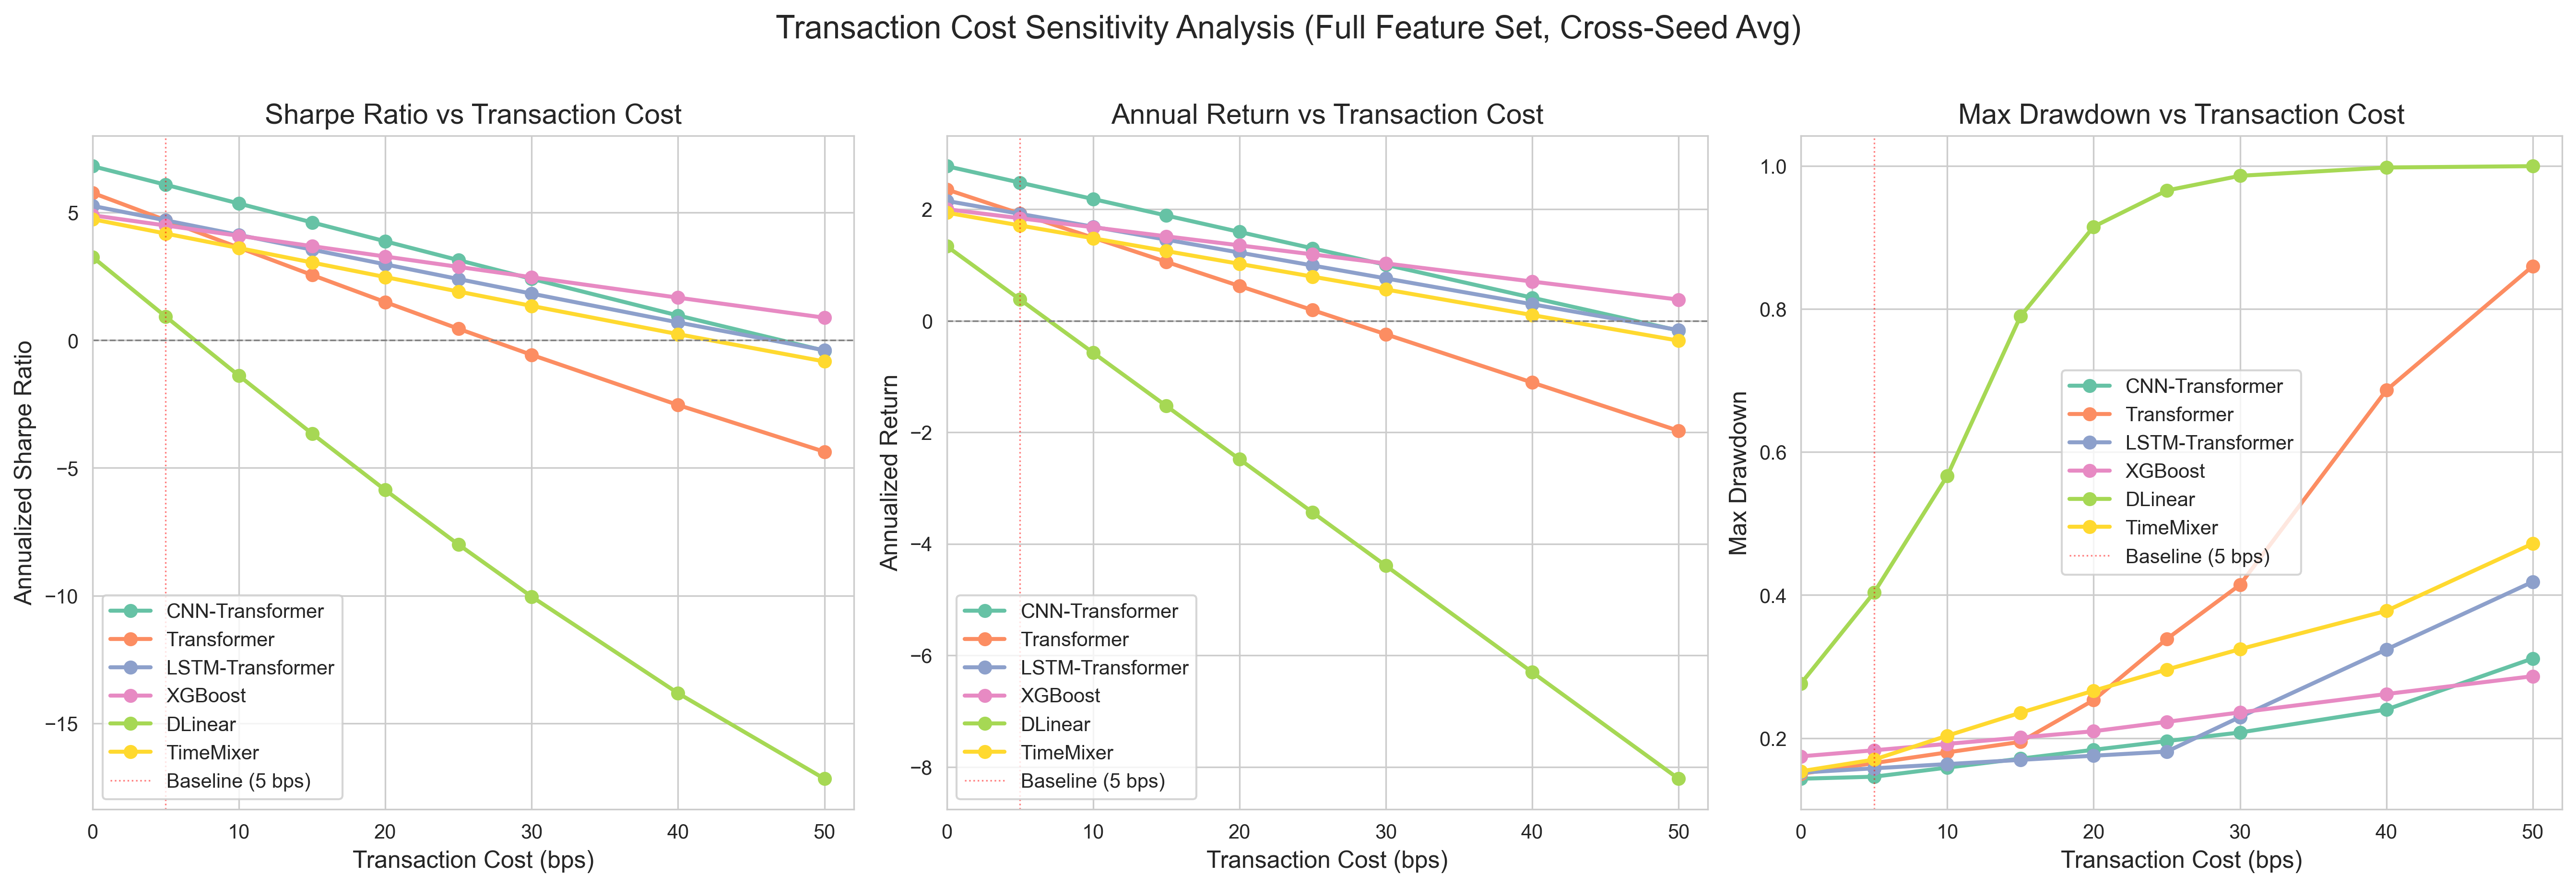
\includegraphics[width=0.95\textwidth]{../charts/cost_sensitivity.png}
    \caption{交易成本敏感性分析（full特征集，跨5种子平均）：从左至右分别为夏普比率、年化收益和最大回撤随手续费（0--50 bps）的衰减曲线}
    \label{fig:cost_sensitivity}
    \end{figure}

    盈亏平衡手续费方面，混合架构（CNN-Transformer 47 bps, LSTM-Transformer 46 bps）显著优于纯Transformer（27 bps）；在20 bps下混合架构的夏普衰减率（36--37\%）远低于纯Transformer（68\%）。TimeMixer展现出意外的成本韧性（盈亏平衡约42 bps），其适中的换手率（11.0\%）限制了交易成本侵蚀。DLinear则因高达46.0\%的换手率（约每9小时翻转一次仓位），盈亏平衡仅约7 bps，成本承受力极弱。换手率数据（表\ref{tab:turnover}）揭示了成本韧性的行为根源：CNN-Transformer的17.9\%换手率处于"中频"最优区间，TimeMixer和LSTM-Transformer以较低换手率（11.0\%、7.9\%）实现更保守的信号生成，纯卷积架构高达26--27\%，而DLinear的46.0\%换手率在扣除交易成本后迅速耗尽策略收益。

    \input{../results/turnover_rates.tex}

    \item \textbf{架构选择的实践启示。}本文的三组分类为实际部署提供了明确的模型筛选依据。若特征集中包含链上数据，应优先选择混合架构（CNN-Transformer、LSTM-Transformer）以充分释放跨源协同效应，二者在成本韧性上也具显著优势（盈亏平衡约47 bps）。若因数据获取成本或推理延迟约束无法引入链上数据，TimeMixer等多尺度混合架构在价格+资金费率+情绪特征组合上表现最优（Sharpe 4.89），且成本韧性意外出色（盈亏平衡约42 bps）。纯注意力架构（Transformer、PatchTST）虽无法利用链上协同，但也不会因链上数据引入而受损，可作为特征集不确定时的"安全默认选择"。纯循环和纯卷积架构在引入链上数据后系统性恶化，应避免在多源异构场景中单独部署。特别地，滑动窗口下XGBoost的崩溃（静态Sharpe 4.50$\to$均值$-0.79$）提醒从业者：树模型的高静态Sharpe可能是"幸运过拟合"的产物，基于滑动窗口的时序交叉验证应成为金融预测模型评估的标准配置。DLinear接近零的跨窗口均值（$-1.26$）也表明，在高度非线性的多源异构场景中，纯线性分解方法的实用性有限。
\end{enumerate}

\section{结论与展望}

本文在比特币4小时K线数据上，通过六种多源异构特征组合和十种模型的交叉实验，系统检验了链上数据在短期收益预测中的有效性及其对模型架构的依赖性。本文的三项核心贡献如下：

\begin{enumerate}[label=(\arabic*),leftmargin=2.5em]
    \item 条件有效性原理：发现链上数据的预测价值是条件性的，而非独立存在的。短期链上指标（SOPR/CDD）在孤立使用时不具备正向预测能力，但与衍生品和情绪特征组合后可产生统计显著的夏普增益。长期链上指标在4小时频率上未展现预测价值。这一发现为业界"全量堆砌"和"完全放弃"链上数据的两种极端实践提供了实证判断依据。
    \item 三组架构分化规律：发现链上协同效应具有清晰的架构依赖性，十种模型呈三组分化——混合架构（CNN-Transformer、LSTM-Transformer）能有效利用链上信号并产生强正向协同（$\Delta$Sharpe $> +2$）；纯注意力架构、线性模型和树模型（Transformer、PatchTST、DLinear、XGBoost）对链上数据呈中性反应（$\Delta$Sharpe $\approx 0$）；纯循环、纯卷积和多尺度混合架构（LSTM、TCN、ModernTCN、TimeMixer）则受到负向干扰（$\Delta$Sharpe $< -1.5$）。这一分组规律在5种子间一致成立，跨滑动窗口保持稳健。TimeMixer作为ICLR 2024 SOTA在price\_funding\_fng上取得全模型最优（Sharpe=4.89），但加入链上数据后崩溃（$\Delta$Sharpe $-$3.11），成为该规律的最有力反证。本文的核心洞察在于特征集$\times$模型架构的交互效应，而非单一模型的绝对排序。
    \item 多维度评估与部署洞察：建立了从预测精度到部署可行性的完整评估链路。发现混合架构的成本韧性约为纯架构的两倍（盈亏平衡约47 bps vs 27 bps），行为根源为适中的换手率水平。滑动窗口验证进一步确认，协同利用组跨8个市场体制的夏普均值最高（3.85），而XGBoost的静态高夏普（4.50）在滑动窗口下完全消失（均值$-0.79$）——这一发现对金融预测模型评估具有方法论层面的警示意义。
\end{enumerate}

本文的局限性及未来方向包括：（1）当前研究仅覆盖BTC单一交易标的，跨资产验证有待开展——ETH等智能合约平台的链上数据具有不同的经济语义（如Gas消耗、DeFi锁仓量），其"链上数据的条件有效性"是否遵循与BTC相似的条件依赖机制尚未可知；传统资产（股票、外汇）则完全缺乏链上数据维度，本文的方法论框架能否部分迁移（如将链上变量替换为资金流或订单流指标）值得探索；（2）当前结论基于4小时单一时间粒度，不同频率下链上数据的有效性可能发生质变——日频或周频上，长期链上指标（交易所余额、活跃地址）的预测价值可能显著上升，因其波动周期与宏观供需节奏更匹配；在1小时或分钟级高频下，市场微观结构噪声可能淹没链上信号，本文的"条件有效性"论断和三类架构分组在不同时间粒度下的稳定性需进一步验证；（3）跨源交互依赖手工交互项，图神经网络可能是更系统化的框架；（4）可探索更贴近实盘的交易模拟（含保证金、仓位约束和滑点）；（5）滑动窗口验证目前仅使用单种子，未来可扩展至多种子。

\newpage

% ================================================================
%  致谢
% ================================================================
\section*{致谢}
本文受教育部人文社科项目（编号：19YJCZH031）和上海市教育科学研究市级项目（编号：C2023068）资助。

% ================================================================
%  参考文献
% ================================================================
\begin{thebibliography}{99}

\bibitem{catania2019}
Catania L, Grassi S, Ravazzolo F.
Predicting the volatility of cryptocurrency time-series.
In \textit{Mathematical and Statistical Methods for Actuarial Sciences and Finance (MAF 2018)}. Springer, 2018: 203--207.
DOI: \href{https://doi.org/10.1007/978-3-319-89824-7\_37}{10.1007/978-3-319-89824-7\_37}.

\bibitem{mcnally2018}
McNally S, Roche J, Caton S.
Predicting the price of Bitcoin using Machine Learning.
In \textit{Proc. 26th Euromicro Int. Conf. Parallel Distrib. Netw.-based Process. (PDP)}, 2018: 339--343.
DOI: \href{https://doi.org/10.1109/PDP2018.2018.00060}{10.1109/PDP2018.2018.00060}.

\bibitem{lim2021}
Lim B, Arik S O, Loeff N, et al.
Temporal Fusion Transformers for interpretable multi-horizon time series forecasting.
\textit{Int. J. Forecast.}, 2021, 37(4): 1748--1764.
DOI: \href{https://doi.org/10.1016/j.ijforecast.2021.03.012}{10.1016/j.ijforecast.2021.03.012}.

\bibitem{nie2023}
Nie Y, Nguyen N H, Sinthong P, Kalagnanam J.
A Time Series is Worth 64 Words: Long-term Forecasting with Transformers.
In \textit{Int. Conf. Learn. Represent. (ICLR)}, 2023.
DOI: \href{https://doi.org/10.48550/arXiv.2211.14730}{10.48550/arXiv.2211.14730}.

\bibitem{luo2024}
Luo D, Wang X.
ModernTCN: A Modern Pure Convolution Structure for General Time Series Analysis.
In \textit{Int. Conf. Learn. Represent. (ICLR)}, 2024.
URL: \href{https://openreview.net/forum?id=vpJMJerXHU}{openreview.net/forum?id=vpJMJerXHU}.

\bibitem{hochreiter1997}
Hochreiter S, Schmidhuber J.
Long Short-Term Memory.
\textit{Neural Comput.}, 1997, 9(8): 1735--1780.
DOI: \href{https://doi.org/10.1162/neco.1997.9.8.1735}{10.1162/neco.1997.9.8.1735}.

\bibitem{vaswani2017}
Vaswani A, Shazeer N, Parmar N, et al.
Attention Is All You Need.
In \textit{Adv. Neural Inf. Process. Syst. (NeurIPS)}, 2017.
DOI: \href{https://doi.org/10.48550/arXiv.1706.03762}{10.48550/arXiv.1706.03762}.

\bibitem{bai2018}
Bai S, Kolter J Z, Koltun V.
An Empirical Evaluation of Generic Convolutional and Recurrent Networks for Sequence Modeling.
\textit{arXiv}, arXiv:1803.01271, 2018.
DOI: \href{https://doi.org/10.48550/arXiv.1803.01271}{10.48550/arXiv.1803.01271}.

\bibitem{chen2016}
Chen T, Guestrin C.
XGBoost: A Scalable Tree Boosting System.
In \textit{Proc. 22nd ACM SIGKDD Int. Conf. Knowl. Discov. Data Min. (KDD)}, 2016: 785--794.
DOI: \href{https://doi.org/10.1145/2939672.2939785}{10.1145/2939672.2939785}.

\bibitem{grinold2000}
Grinold R C, Kahn R N.
\textit{Active Portfolio Management: A Quantitative Approach for Providing Superior Returns and Controlling Risk}. 2nd ed. McGraw-Hill, 2000.
ISBN: 978-0070248823.

\bibitem{diebold1995}
Diebold F X, Mariano R S.
Comparing Predictive Accuracy.
\textit{J. Bus. Econ. Stat.}, 1995, 13(3): 253--263.
DOI: \href{https://doi.org/10.1080/07350015.1995.10524599}{10.1080/07350015.1995.10524599}.

\bibitem{ledoit2008}
Ledoit O, Wolf M.
Robust Performance Hypothesis Testing with the Sharpe Ratio.
\textit{J. Empir. Finance}, 2008, 15(5): 850--859.
DOI: \href{https://doi.org/10.1016/j.jempfin.2008.03.002}{10.1016/j.jempfin.2008.03.002}.

\bibitem{omole2024}
Omole O, Enke D.
Deep learning for Bitcoin price direction prediction: models and trading strategies empirically compared.
\textit{Financ. Innov.}, 2024, 10: 117.
DOI: \href{https://doi.org/10.1186/s40854-024-00643-1}{10.1186/s40854-024-00643-1}.

\bibitem{kozh2025}
Kozhevnikov V.
Machine Learning techniques for predictive modeling of Bitcoin price dynamics.
Master's thesis, Prague University of Economics and Business (VŠE), 2025.
URL: \href{https://vskp.vse.cz/98304}{vskp.vse.cz/98304}.

\bibitem{kim2022}
Kim G, Shin D, Choi J G, Lim S.
A deep learning-based cryptocurrency price prediction model that uses on-chain data.
\textit{IEEE Access}, 2022, 10: 56232--56248.
DOI: \href{https://doi.org/10.1109/ACCESS.2022.3177888}{10.1109/ACCESS.2022.3177888}.

\bibitem{pambudi2025}
Pambudi R, Nugraheni D M K, Widodo A P.
Comparative Performance Analysis of Deep Learning Models for Cryptocurrency Price Forecasting.
\textit{Sci. J. Inform.}, 2025, 12(4): 743--756.
DOI: \href{https://doi.org/10.15294/sji.v12i4.35653}{10.15294/sji.v12i4.35653}.

\bibitem{findev2025}
Hasanli R, Dursun M.
Integrating high-dimensional technical indicators into machine learning models for predicting cryptocurrency price movements and trading performance: evidence from Bitcoin, Ethereum, and Ripple.
\textit{FinTech}, 2025, 4(4): 77.
DOI: \href{https://doi.org/10.3390/fintech4040077}{10.3390/fintech4040077}.

\bibitem{urquhart2016}
Urquhart A.
The inefficiency of Bitcoin.
\textit{Econ. Lett.}, 2016, 148: 80--84.
DOI: \href{https://doi.org/10.1016/j.econlet.2016.09.019}{10.1016/j.econlet.2016.09.019}.

\bibitem{alessandretti2018}
Alessandretti L, ElBahrawy A, Aiello L M, Baronchelli A.
Anticipating Cryptocurrency Prices Using Machine Learning.
\textit{Complexity}, 2018, 2018: 8983590.
DOI: \href{https://doi.org/10.1155/2018/8983590}{10.1155/2018/8983590}.

\bibitem{kristoufek2015}
Kristoufek L.
What Are the Main Drivers of the Bitcoin Price? Evidence from Wavelet Coherence Analysis.
\textit{PLOS ONE}, 2015, 10(4): e0123923.
DOI: \href{https://doi.org/10.1371/journal.pone.0123923}{10.1371/journal.pone.0123923}.

\bibitem{corbet2019}
Corbet S, Lucey B, Urquhart A, Yarovaya L.
Cryptocurrencies as a financial asset: A systematic analysis.
\textit{Int. Rev. Financ. Anal.}, 2019, 62: 182--199.
DOI: \href{https://doi.org/10.1016/j.irfa.2018.09.003}{10.1016/j.irfa.2018.09.003}.

\bibitem{cerqueira2020}
Cerqueira V, Torgo L, Mozeti\v{c} I.
Evaluating time series forecasting models: an empirical study on performance estimation methods.
\textit{Data Min. Knowl. Discov.}, 2020, 34: 1356--1389.
DOI: \href{https://doi.org/10.1007/s10618-020-00694-1}{10.1007/s10618-020-00694-1}.

\bibitem{carosia2024}
Carosia A E O, Coelho G P, Silva A E A.
Bitcoin price prediction based on fear \& greed index.
In \textit{SHS Web Conf.}, 2024, 188: 02015.
DOI: \href{https://doi.org/10.1051/shsconf/202418802015}{10.1051/shsconf/202418802015}.

\bibitem{malik2023}
Malik A.
A comparison of machine learning and econometric models for pricing perpetual Bitcoin futures and their application to algorithmic trading.
\textit{Expert Syst.}, 2023, 40(10): e13414.
DOI: \href{https://doi.org/10.1111/exsy.13414}{10.1111/exsy.13414}.

\bibitem{wen2023}
Wen Q, Zhou T, Zhang C, Chen W, Ma Z, Yan J, Sun L.
Transformers in Time Series: A Survey.
\textit{arXiv:2202.07125}, 2023. (Appeared at IJCAI 2023).

\bibitem{das2026}
Das B, Dagdogen H A, Kaya M O, Das R.
A new hybrid approach combining transformer-based language models and graph neural networks for cryptocurrency forecasting.
\textit{Eng. Appl. Artif. Intell.}, 2026, 164: 113179.
DOI: \href{https://doi.org/10.1016/j.engappai.2025.113179}{10.1016/j.engappai.2025.113179}.

\bibitem{zeng2023}
Zeng A, Chen M, Zhang L, Xu Q.
Are Transformers Effective for Time Series Forecasting?
In \textit{Proc. AAAI Conf. Artif. Intell. (AAAI)}, 2023, 37(9): 11121--11128.
DOI: \href{https://doi.org/10.1609/aaai.v37i9.26317}{10.1609/aaai.v37i9.26317}.

\bibitem{wang2024timemixer}
Wang S, Wu H, Shi X, Hu T, Luo H, Ma L, Zhang J Y, Zhou J.
TimeMixer: Decomposable Multiscale Mixing for Time Series Forecasting.
In \textit{Int. Conf. Learn. Represent. (ICLR)}, 2024.
URL: \href{https://openreview.net/forum?id=7oLshfEIC2}{openreview.net/forum?id=7oLshfEIC2}.

\end{thebibliography}

\end{document}
